\externaldocument{chapter2} 
\chapter{Literature Review}
\label{chap:softwareTesting}
The famous quote of Paul Ehrlich, ``to err is human, but to really foul things up you need a computer", is quite relevant to the software programmers. Programmers being humans are prone to errors. In spite of their best efforts, some errors may remain in the software after it is finalised.  Errors cannot be tolerated in software because a single error may cause a large upset in the system. The destruction of Mariner 1 rocket (1962) due to unit conversion error costing \$18.5 million, Hartford Coliseum Collapse (1978) costing \$70 million, Wall Street crash (1987) costing \$500 billion, failing of long division by Pentium\texttrademark (1993) costing \$475 million, Ariane 5 Rocket disaster (1996) costing \$500 million and many more were caused by minor errors in the software \cite{garfinkel2005history, toweysoftware}. According to the National Institute of Standards and Technology, US companies alone bear \$59.5 billion loss every year due to software failures and one-third of that can be eliminated by improving the testing infrastructure~\cite{tassey2002economic}. To achieve high quality, a piece of software has to satisfy rigorous stages of testing. The more complex the software, the higher the requirements for software testing and the larger the damage caused when a bug remains in the software.

\section{Software Testing}
According to the IEEE standard glossary of software engineering~\cite{american1984}, testing is defined as, ``the process of exercising or evaluating a system or system component by manual or automated means to verify that it satisfies specified requirements or to identify differences between expected and actual results". The process of software testing in its simplest form is shown in Figure~\ref{fig:softwareTestingParts_2}. 

\begin{figure}[h]
	\centering
	\centerline{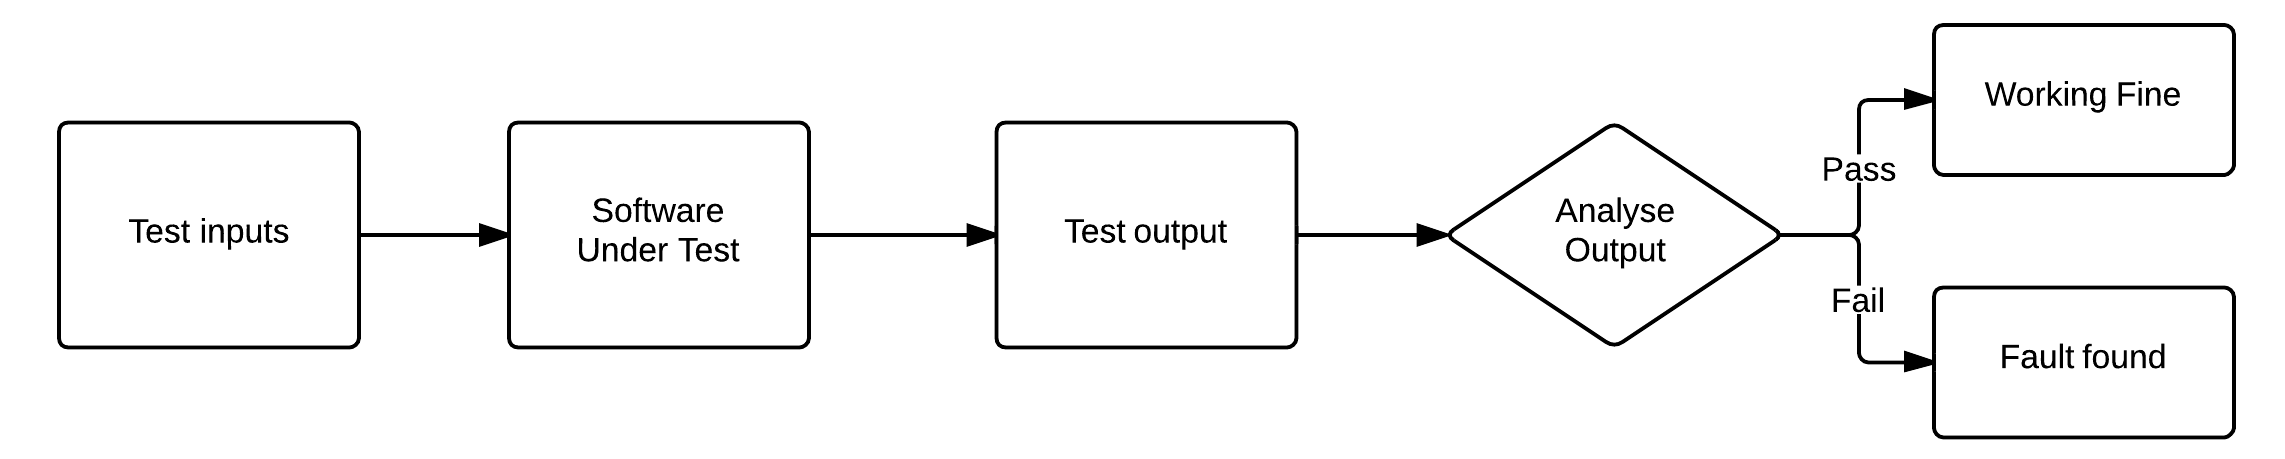
\includegraphics[width=16cm, height=5cm]{chapter2/softwareTesting.png}}
	\caption{A simplified version of software testing process}
	\label{fig:softwareTestingParts_2}
\end{figure}

The testing process, being an integral part of Software Development Life Cycle (SDLC), starts from requirement phase and continues throughout the life of the software according to a predefined test plan. Test plan is a document which defines the goal, scope, method, resources and time schedule of testing \cite{futrell2001quality}. In addition, it includes the testable deliverables and the associated risk assessment. The test plan explains \verb+who, when, why+ and \verb+how+ to perform a specific activity in the testing process. 

In traditional testing, when testers find a fault, the software is returned to the developers for rectification and consequently given back to the testers for retesting. It is important to note that a successful test is the one that fails a software or identifies fault in the software~\cite{myers2011art}. Fault denotes error made by programmers during software development~\cite{american1984}. The faulty code on execution can lead to software failures. A software that passes all the tests without giving a single error is not guaranteed to contain no error. However, the testing process increases reliability and confidence of users in the tested product~\cite{dahl1972structured}. Software testing from various view points is presented in Figure~\ref{fig:softwareTestingFlow_2}.


\begin{figure}[H]
	\centering
	%\centerline{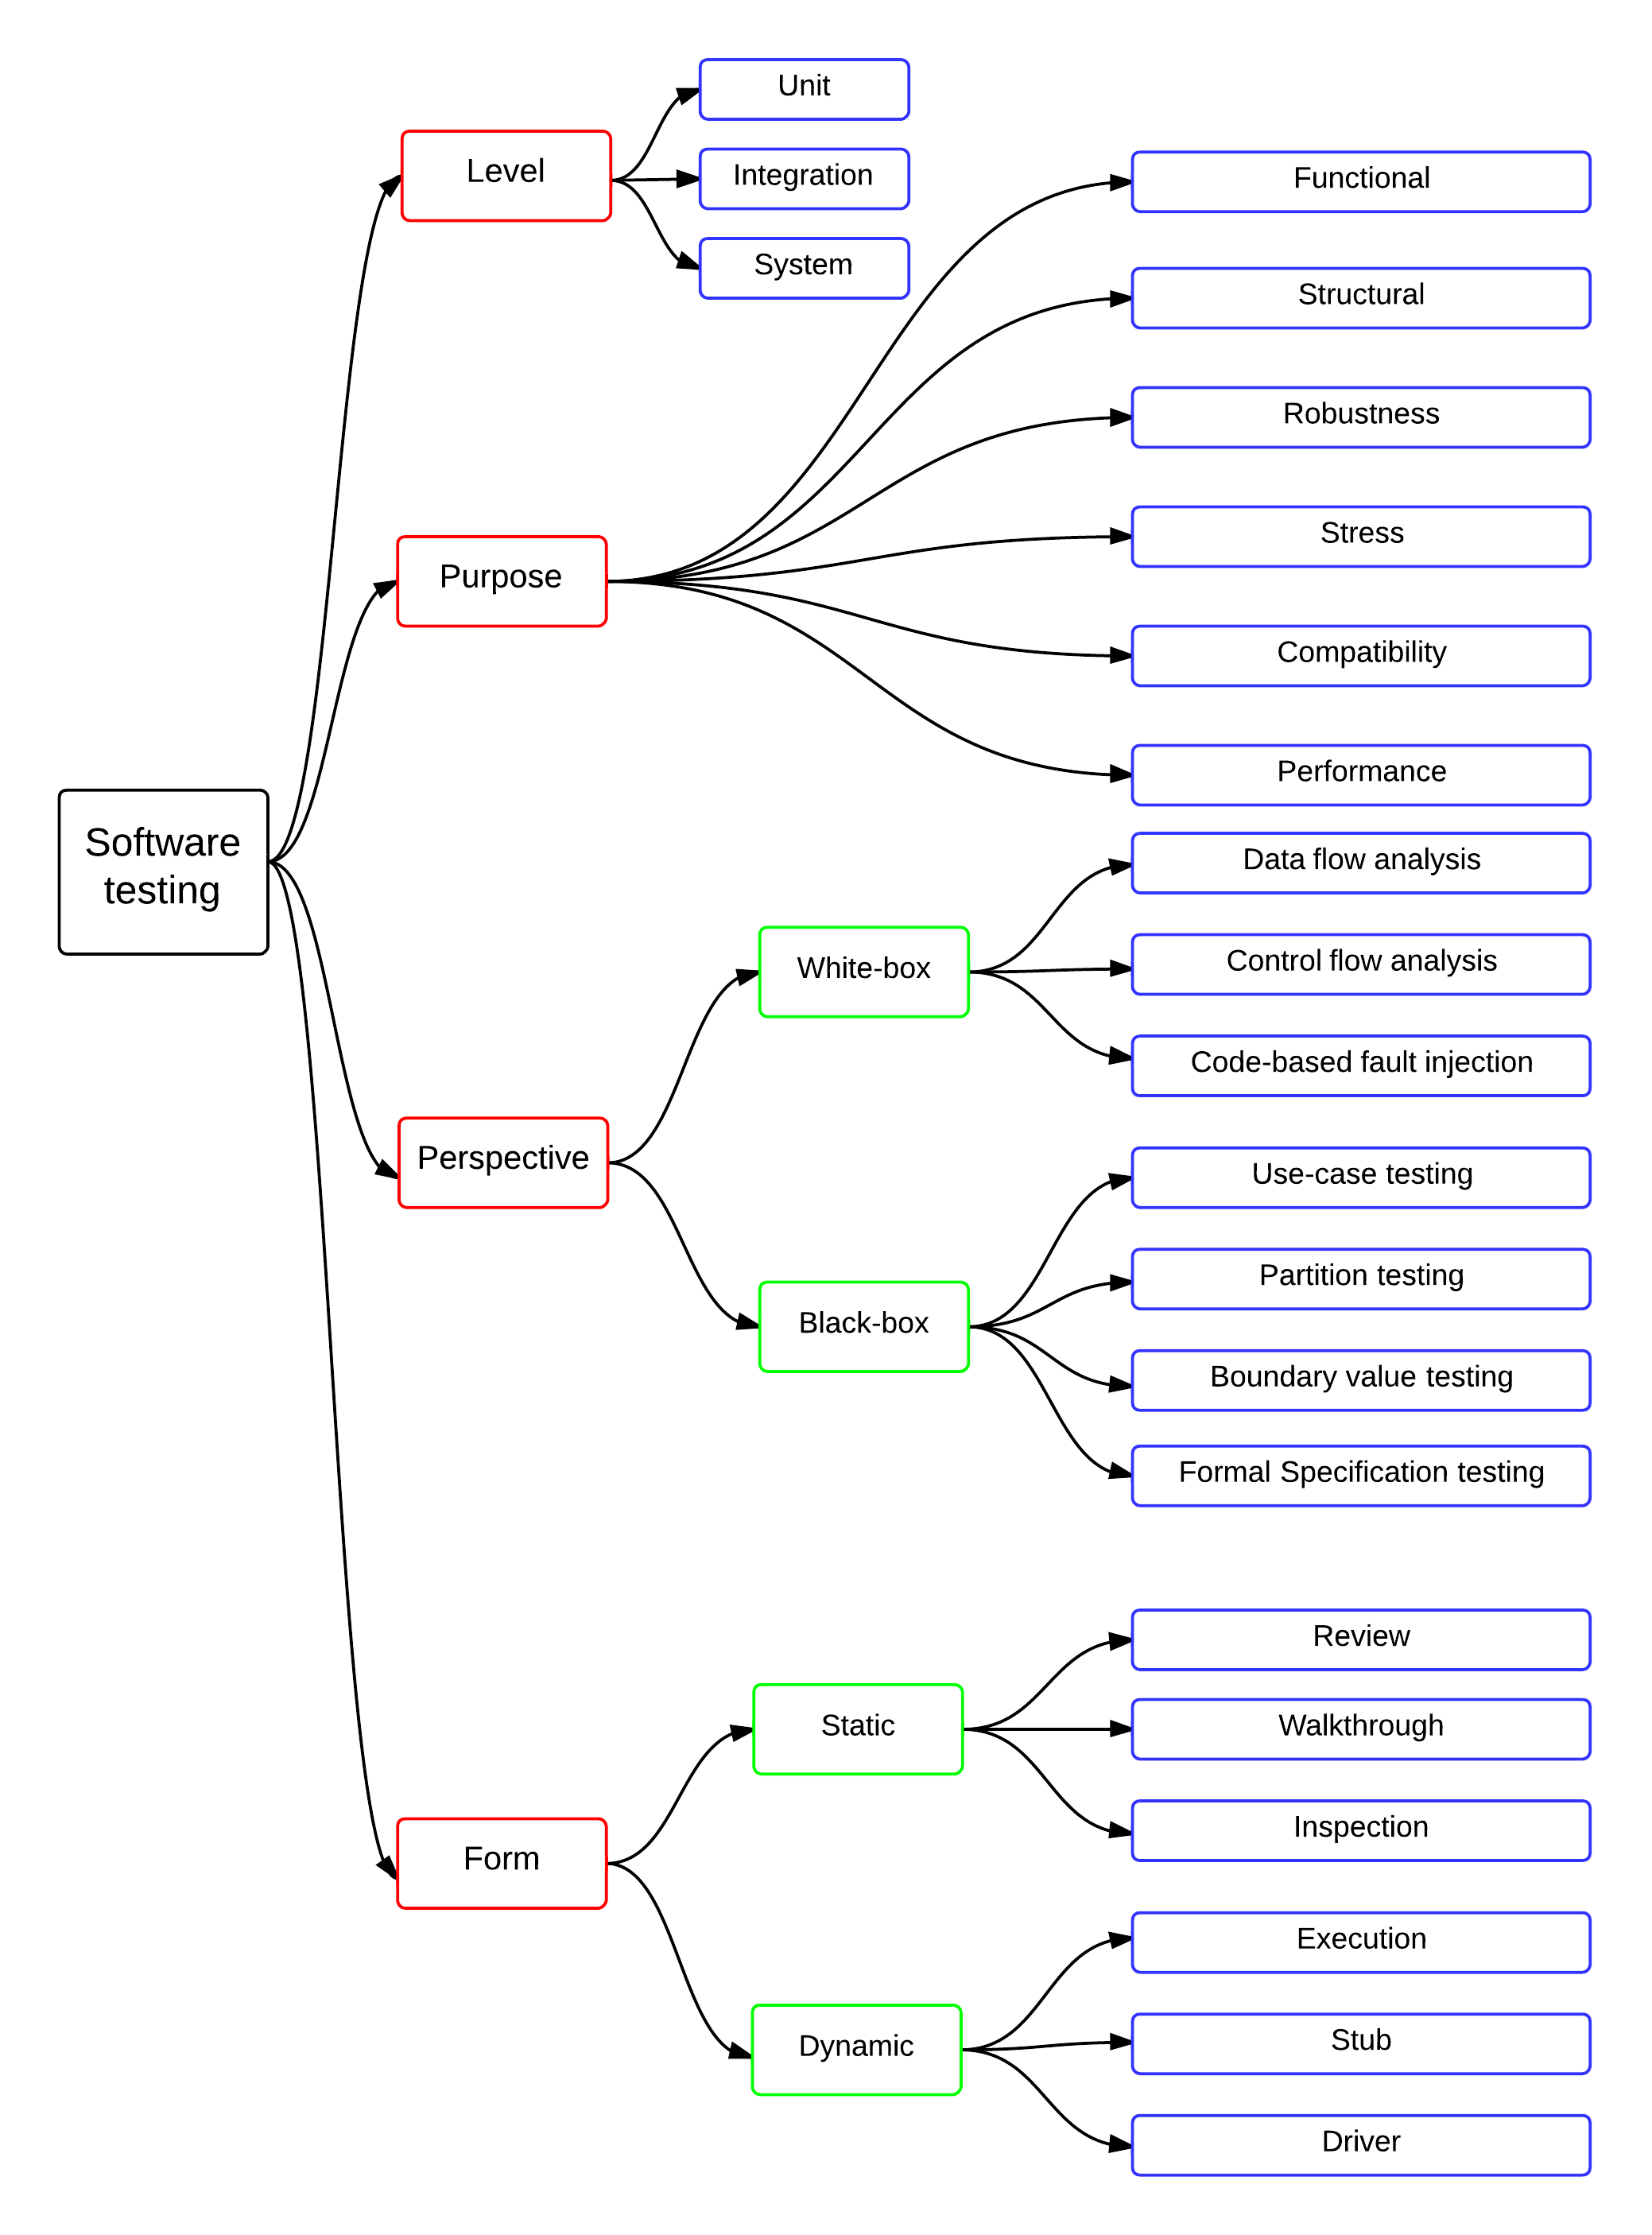
\includegraphics[width=16cm, height=16cm]{chapter2/softwareTestingFlow.png}}
	\centerline{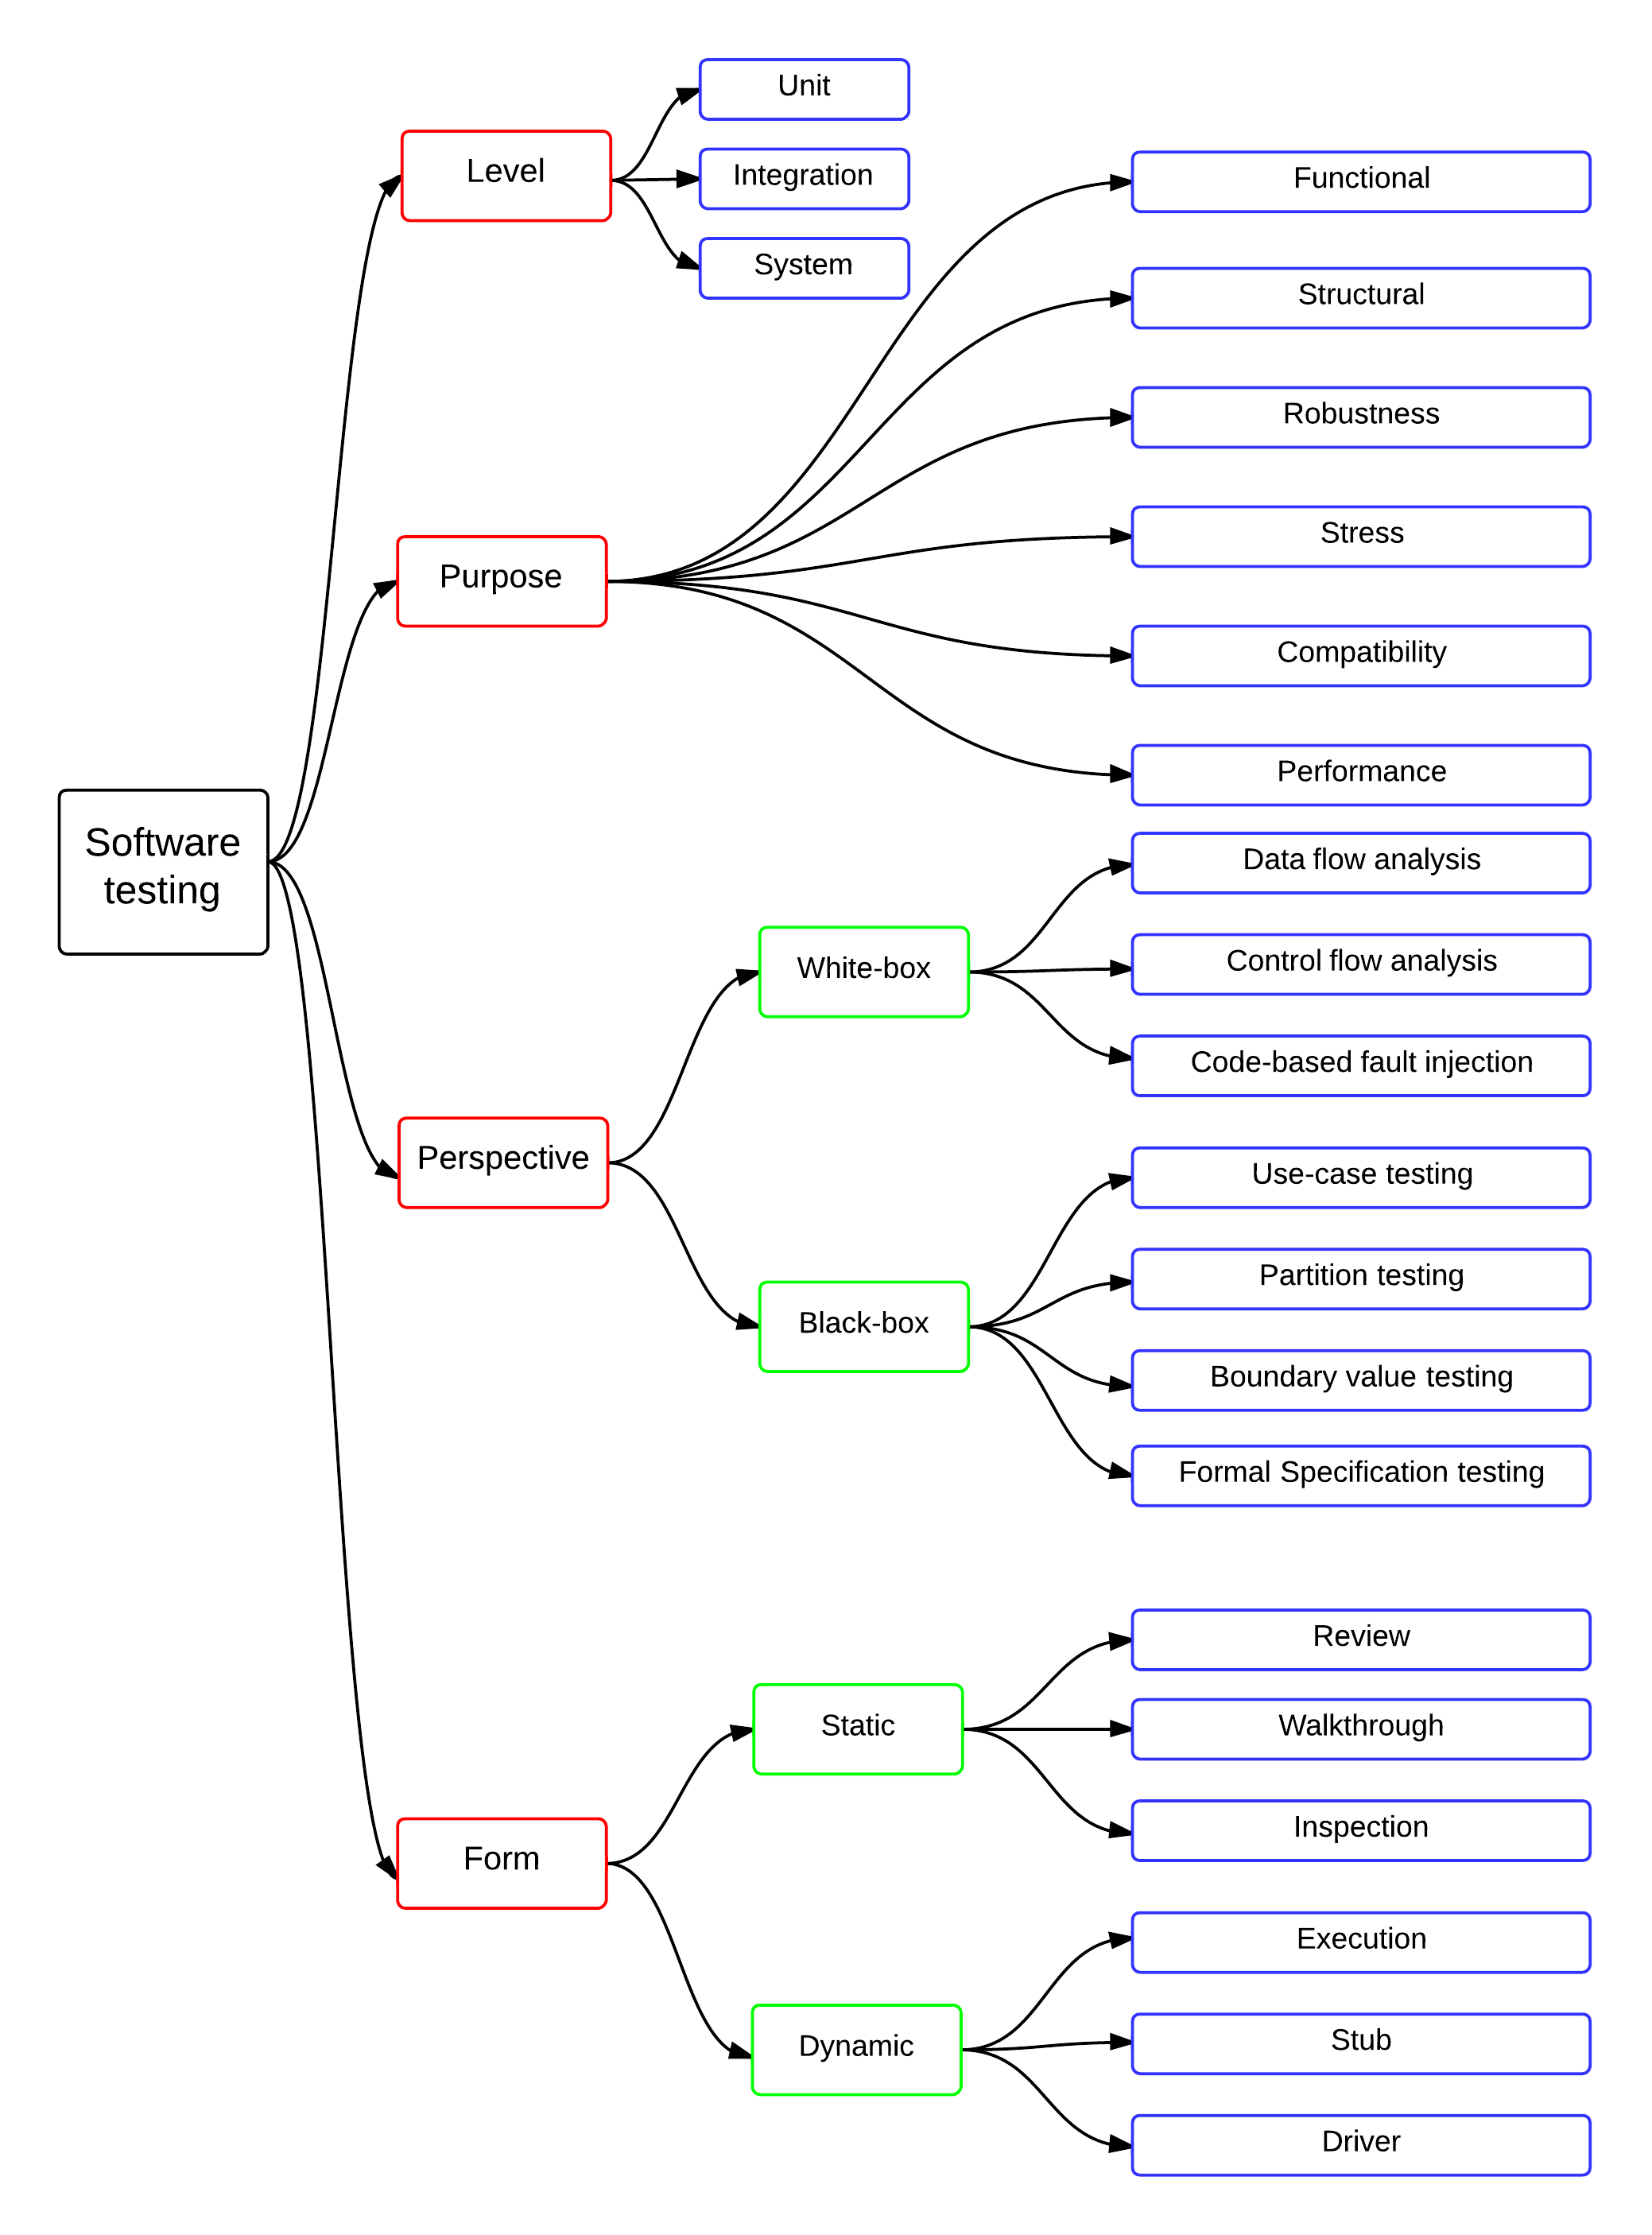
\includegraphics[width=\textwidth]{chapter2/softwareTestingFlow.png}}
	\caption{Software testing from various view points}
	\label{fig:softwareTestingFlow_2}
\end{figure}



%\begin{table}[ht]
%%\scriptsize
%\caption{Parts of Software Testing} % title of Table
%\bigskip
%\centering % used for centering table
%{\renewcommand{\arraystretch}{1.5} %<- modify value to suit your needs
%\begin{tabular}{| l | l | l | l | } % centered columns (4 columns)
%\hline
%
%Level 					&Purpose		 		& Perspective					& Form 					\\
%\hline
%Unit					& Functional			& White Box							& Static 					\\
%Integration				& Structural			& ~~~~Data Flow Analysis				& ~~~~Reviews			\\
%System					& Robustness		& ~~~~Control Flow Analysis			& ~~~~Walkthroughs		\\
%						& Stress				& ~~~~Code-based fault injection 		& ~~~~Inspection		\\
%						& Compatibility		& Black Box							& Dynamic				\\
%						& Performance		& ~~~~Use-case testing				& ~~~~Execution			\\
%						&					& ~~~~Partition testing				& ~~~~Stubs				\\
%						&					& ~~~~Boundary Value testing			& ~~~~Drivers			\\
%						&					& ~~~~Formal Specification testing		&						\\
%
%
%
%\hline %inserts single line
%\end{tabular}
%}
%\bigskip
%\label{table:softwareTestingParts} % is used to refer this table in the text
%\end{table}



\section{Software Testing Levels}
Unit testing, Integration testing and System testing are the three main levels of software testing reported in the literature~\cite{chilenski1994applicability}. Unit testing deals with evaluation of code piece-by-piece and each piece is considered as independent unit. Units are combined together to form components. Integration testing is performed to make sure that integration of units in a component are working properly. System testing ensures that the system formed by the combination of components proceeds properly to give the required output.

\section{Software Testing Purpose}
The purpose of software testing is identification of faults in the given SUT for necessary correction in order to achieve high quality. Maximum number of faults can be identified if software is tested exhaustively. However, exhaustive testing is not always possible because of limited resources and infinite number of input values that a software can take. Therefore, the purpose of testing is generally directed to achieve confidence in the system involved from a specific point of view. For example, functionality testing is performed to check that functional aspect are working correctly. Structural testing analyses the code structure for generating test cases in order to evaluate paths of execution and identification of unreachable or dead code. Robustness testing observes the software behaviour when software receives input outside the expected input range. Stress and performance testing aims at testing the response of software under high load and checking its ability to process different nature of tasks~\cite{cohen2005robustness}. Compatibility testing is performed to see the interaction of software with the underlying operating system.
 %As proper planning is the key to success for many projects this is often also true with software testing. A software test plan is a well defined document that defines the goal, scope, method, resources and time schedule of the testing.
%A software testing technique in which a software is tested with all possible combination of inputs. This technique can prove conclusively that the software meet its specification however exhaustive testing is seldom feasible because of the large input domain or too many paths in a software code. 

\section{Software Testing Perspective}
Software testing is divided into white-box and black-box testing based on the perspective taken.

\subsection{White-box Testing}
\begin{wrapfigure}{r}{0.36\textwidth}
  \vspace{-35pt}
  \begin{center}
   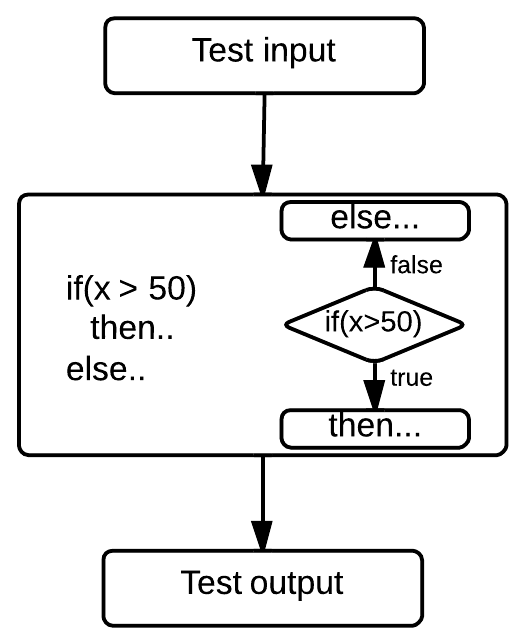
\includegraphics[width=0.30\textwidth]{chapter2/whiteBox.png}
  \end{center}
  \vspace{-20pt}
  \bigskip
  \caption{White-box testing}
 \vspace{-18pt}
\end{wrapfigure}
In white-box or structural testing, the testers must know about the complete structure of the software so that they may be able to make necessary modifications, if so required. Test cases are derived from the code structure and test passes if the results are correct and the proper code is followed during test execution~\cite{ostrand2002white}. Some commonly used white-box testing techniques are as follows:
%\begin{figure}[h]
%\begin{center}
%	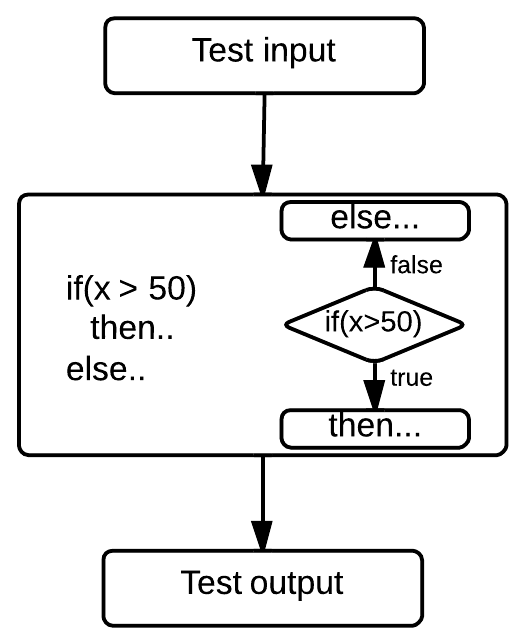
\includegraphics[width=5cm, height=5.5cm ]{chapter2/whiteBox.png}
%	\caption{White-box testing}
%	\label{fig:blackBox}
%\end{center}  
%\end{figure}


\subsubsection{Data Flow Analysis}
Data Flow Analysis (DFA) is a technique which focuses on the input values by observing the behaviour of respective variables during execution of the SUT~\cite{clarke1989formal}. In this technique a Control Flow Graph (CFG), graphically representing all possible states of a program, is drawn to determine the paths that are traversed by the program during test execution. Test cases are generated and executed to verify conformance with CFG. 

The data flow analysis observes the program execution as data-flow from input to output.
The data may transform into several intermediary steps before reaching the final state. The process is prone to several errors e.g. references made to non existing variables, values assigned to undeclared variables or change of variables in undesired manner. Ordered use of data is crucial to ensure that the aforementioned errors do not occur~\cite{fosdick1976data}.

\subsubsection{Control Flow Analysis}
Control Flow Analysis (CFA) is a technique which takes into consideration the control structure of a given SUT. Control structure is the order in which the statements, instructions and function calls are executed. In this technique a CFG, similar to the one required in DFA, is drawn to determine the traversable paths by a program during the execution. Test cases are generated and executed to verify conformance with CFG on the basis of control. Taking the example of following a specific path between two or more available choices at a particular state, efforts are made to ensure that the set of selected test cases execute all the possible control choices at least once. Two of the most common measurement criteria defined by Vilkomir et al. are Branch coverage and Condition coverage~\cite{vilkomir2003tolerance}. 

\subsubsection{Code-based Fault Injection Testing}
It is a testing technique in which new instructions are added to the code of the SUT at one or more locations to analyse the software behaviour in response to the given instructions. \cite{voas1997software}. The process of code addition (instrumentation) is performed before compilation and execution of software. Code is added to find error handling behaviour of software, examine the capability of test procedure and measure the code coverage achieved by the testing process.    

\subsection{Black-box Testing}
\begin{wrapfigure}{r}{0.36\textwidth}
  \vspace{-35pt}
  \begin{center}
    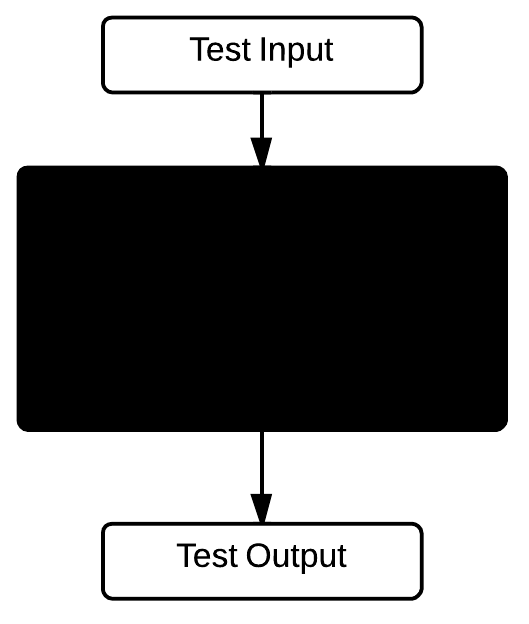
\includegraphics[width=0.30\textwidth]{chapter2/blackBox.png}
  \end{center}
  \vspace{-20pt}
  \bigskip
  \caption{Black-box testing}
  \label{fig:blackBox}
  \vspace{-18pt}
 \end{wrapfigure}
In black-box or functional testing, the testers do not need to know about the internal code structure of the SUT. Test cases are derived from the software specifications and test passes if the result is according to expected output irrespective of the internal code followed during test execution~\cite{beizer1995black}. Some commonly used black-box testing techniques are as follows.
%\begin{figure}[h]
%\begin{center}
%	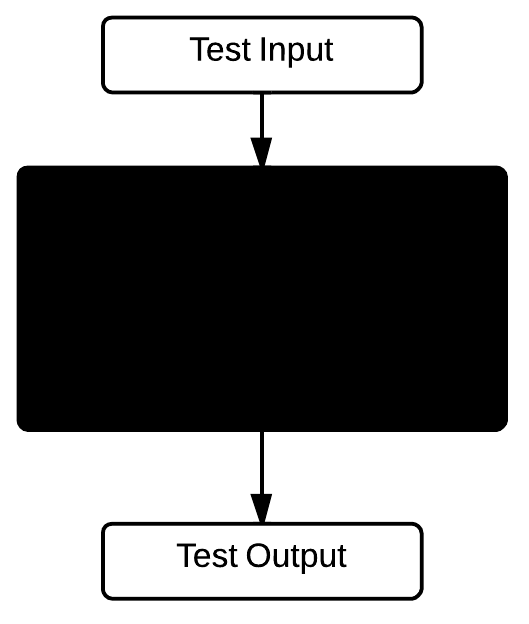
\includegraphics[width=5cm, height=5.5cm ]{chapter2/blackBox.png}
%	\caption{Black-box testing}
% 	\label{fig:blackBox}
%\end{center}  
%\end{figure}



\subsubsection{Use-case Based Testing}
% check if it is use case-based testing or use case testing.
It is a testing technique which utilizes use-cases of the system to generate test cases. Use-case defines functional requirement at a particular point in the system from actor's perspective. It consists of a sequence of actions to represent a particular behaviour of the system. A use-case format includes brief description and flow of events, pre-conditions, post-conditions, extension points, context and activity diagrams. The use-case contains all the information required for test case, therefore, it can be easily transformed into a test case~\cite{armour2000advanced}. Use-case testing is beneficial in terms of cheap generation of test cases, avoidance of test duplication, increased test coverage, easier regression testing and early identification of missing requirements.  

% steps taken from presentation of Raional User Conference 2003. Check it for viva.
\subsubsection{Partition Testing}
It is a testing technique in which the input domain of a given SUT is divided into equal sub-domains for testing each sub-domain individually. The division is based on software specifications, code structure and the process involved in software development~\cite{hamlet1990partition}. The performance of partition testing is directly proportional to the quality of sub-domain~\cite{weyuker1991analyzing}. Division of input domain into equal partitions is often difficult. To overcome the problem, a new version of partition testing, called proportional partition testing~\cite{chan1996proportional} is devised. In this version, the sub-domains vary in size and the number of test cases selected from each partition is directly proportional to the size of the partition. Experiments performed by Ntafos~\cite{ntafos1998random} have provided evidence for better performance of proportional partition testing.


\subsubsection{Boundary Value Analysis}
Boundary Value Analysis (BVA) is a testing technique based on the assumption that errors often reside along the boundaries of the input variables. Thus border values are taken as the test data set in BVA. According to IEEE standards~\cite{radatz1990ieee}, boundary values contain minimum, maximum, internal and external values specified for a system. 

BVA and partition testing may be used in combination by choosing test values from the whole input domain and also from the borders of each sub-domain. Reid et al. \cite{reid1997empirical} have provided evidence in support of better performance of BVA compared to partition testing. However, they have indicated that better performance of BVA is based on accurate identification of partition and selection of boundary values. The following code illustrates the ability of BVA to find a bug. 

\begin{lstlisting}
 public void test (int arg) {
	arg = arg + 1;
	int [] intArray = new intArray[arg];
	...
 }
\end{lstlisting}

On passing interesting value \verb+MAX_INT+ as argument to the \verb+test+ method, the code in the method increment it by 1 making it a negative value and thus an error is generated when the SUT tries to set the array size to a negative value.

\subsubsection{Formal Specification Testing}
It is a testing technique based on mathematical model which provides the opportunity to handle the specifications mechanically. This feature facilitates the isolation, transformation, assembly and repackaging of the information available in the specifications for use as test cases~\cite{donat1997automating}.

The formal specification testing is more productive because of the creation of test cases independent from the code of the SUT~\cite{gaudel2010software}. The extra effort of generating test oracle is avoided because of using the available specification model for verifying the test results~\cite{bertolino2007software}.
  

%\section{Common Techniques of Software Testing}
%This section briefly define some of the most common techniques of software testing currently being used in the testing industry. These include techniques from both white-box and black-box testing techniques.

% Check wikipedia for them.


%\subsubsection{Grey-Box Testing}
%Grey-Box testing is the combination of both black-box/functionality and white-box/structural testing. The tester knows about both the functionality and the internal structure of the SUT. Some of the test cases are based on the functionality and some of the test cases are based on the structure. Emphasis of grey-box testing is both on code coverage as well as functionality~\cite{Savenkov2008}.

%\subsection{Software Testing Workflow}
%There are many software techniques like unit testing, integration testing, random testing, regression testing, system testing, acceptance testing, performance testing, load testing, stress testing, alpha testing, beta test etc. All testing techniques belong to black-box, white-box or grey-box approach. Each testing technique has its own strength and weaknesses but the technique in focus here is Random Testing.


%\begin{figure}[h]
%\begin{center}
%	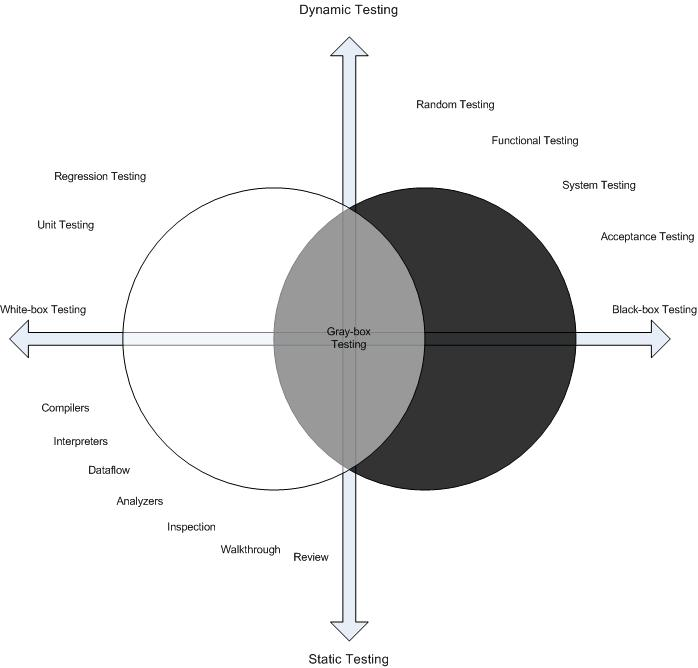
\includegraphics[width=16cm, height=12cm ]{Literature/Drawing34.jpg}
%	\caption{Software Testing Workflow}
%\end{center}  
%\end{figure}


%We have explained software testing graphically with the help of plotting venn diagram on two dimensional axis. The positive x axis represent black-box while negative x axis represent white-box testing. Grey-box testing in the middle is represented by the overlapping of black-box and white-box testing. Similarly on positive y axis we have dynamic testing and on negative y axis we have static testing.
%Now if a test is black box and dynamic then the test will fall in 0 to 90 degree on the diagram and if the test is black-box and static then it will fall in 270 to 360 degree. On the other hand if the test is white-box and dynamic then it will fall in 90 to 180 degree and if the test is white-box and static then it will fall in 180 to 270 degrees.

%\subsection{Automated Test Generation}
%\subsection{Generation Strategies}

\subsection{Test Case}
%\begin{wrapfigure}{r}{0.35\textwidth}
%  \vspace{-20pt}
%  \begin{center}
%    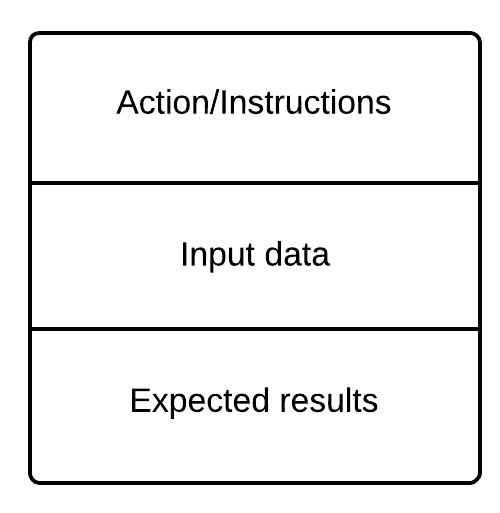
\includegraphics[width=0.30\textwidth]{chapter2/testCase.png}
%  \end{center}
%  \vspace{-20pt}
%  \caption{Test case}
%  \label{fig:testCase}
%  \vspace{-10pt}
%\end{wrapfigure}
A test case is an artifact which delineates the input, action and expected output corresponding to that input \cite{ahmed2010software}. After executing the test case, if the output obtained comply with the expected output, the test case is declared pass which means that the functionality is working correctly, otherwise the test case is declared fail, which represents identification of fault. A series of test cases, also known as test suite, are usually required to be executed for establishing the desired level of quality.


\subsection{Test Oracle}
Test oracle is defined as, ``a source containing expected results for comparison with the actual result of the SUT" \cite{ahmed2010software}. For a program P, an oracle is a function which verifies that the output from P is the same as the output from a ‘correct’ version of P~\cite{howden1986functional}. Test oracle sets the acceptable behaviour for test execution~\cite{baresi2001test}. 

All software testing techniques depend on the availability of test oracle~\cite{gaudel2010software}. Designing test oracle for ordinary software may be simple and straightforward. However, for relatively complex software, designing of oracle is quite cumbersome and requires special ways to overcome the oracle problem. Some of the common oracle problems are as follows:

\begin{enumerate}
\item It is assumed that the test results are observable and comparable with the oracle~\cite{weyuker1982testing}.
\item Ideally, test oracle would satisfy desirable properties of program specifications~\cite{baresi2001test}.
\item A test oracle to satisfy all conditions is seldom available as rightly pointed out by Weyuker, ``truly general test oracles are often unobtainable''~\cite{weyuker1982testing}. 
\end{enumerate}
\bigskip
Post-conditions of a method are the most commonly used test oracle in automated software testing. Post-conditions are conditions which must be true after a method is executed. In such oracle a fault is signalled when a post-condition is violated \cite{meyer2009programs}. Some common artefacts used as oracles are as follows:

\begin{enumerate}
\item Specification and documentation to generate test oracle. 
\item Products similar to the SUT but different in algorithm. %to solve the similar problem.
\item Heuristic algorithms to provide exact results for a set of test cases. % Hoffman, Douglas; Heuristic Test Oracles, Software Testing & Quality Engineering Magazine, 1999
\item Statistical characteristics to generate test oracle. % \cite{mayer2004test}. 
\item Comparison of the result of one test to another for consistency. % Hoffman, Douglas; Analysis of a Taxonomy for Test Oracles, Quality Week, 1998
\item Models to generate test oracle for verification of SUT behaviour. % \cite{robinson1999finite}.
\item Manual analysis by human experts to verify the test results. %\cite{jalote1997integrated}. 
\end{enumerate}

\section{Forms of Software Testing}
There are two forms of software testing: static and dynamic. \\*
In static testing, test cases are analysed statically for checking errors without test execution. In addition to software code, high quality software are supplied with documentation including requirements, design, user manual, technical notes and marketing information. Reviews, walkthroughs and inspections are most commonly used techniques for static testing.\\*
In dynamic testing the software code is executed and input is converted into output. Results are analysed against expected outputs to find any error in the software. Unit testing, integration testing, system testing, and acceptance testing are most commonly used methods for dynamic testing~\cite{fairley1978tutorial}.

%Dynamic testing can be manual or automated. In manual testing the programmer develops the test cases which are executed by the developed software to find any error in processing or output. Similarly in automated testing the software or components of the software is given as input to testing software that automatically generates test cases and executes the SUT against them to find any errors. Manual testing typically consumes more time and resources than automated testing.

\subsection{Manual Software Testing}
Manual testing is the technique in which the tester writes the code manually to create test cases and test oracles for finding faults in software~\cite{ciupa2008finding}. It may be effective at smaller scale but is generally laborious, time consuming and error-prone~\cite{tretmans2000automatic}. In manual testing, testers must have appropriate skills, experience and knowledge of the SUT for evaluation from different perspectives.
 
\subsection{Automated Software Testing}
Automated testing is the technique in which a testing tool is used to perform the testing process automatically for finding faults in software~\cite{leitner2007reconciling}. There are tools for automating a part of testing process like generation of test cases or execution of test cases or evaluation of results. Other tools are available for automating the whole testing process. 
%Increase in functionality, higher productivity and lower cost of production without compromising quality are the desirable features in favour of automating the process of software testing. 
Automated software testing may involve higher initial cost but brings the key benefits of lower cost of production, higher productivity, maximum availability, greater reliability, better performance and ultimately proves highly beneficial for any organisation. Automated testing is particularly effective when the nature of job is repetitive and it is performed on routine basis like unit testing and regression testing where the tests are re-executed after each modification~\cite{huang2003automated}. The use of automated software testing makes it possible to test large volumes of code, which may be impossible otherwise~\cite{ramamoorthy1975testing}.

\section{Test Data Generation}
Test data generation in software testing is the process of identifying input data which satisfies the given selection criterion. A test data generator is used to assist testers in the generation of data while the selection criterion defines the properties of test cases to be generated based on the test plan and perspective taken \cite{korel1990automated}. Various artefacts of the SUT can be considered to generate test data like requirements, model, code etc. The choice of artefacts selected limits the kind of test selection criteria that can be applied in guiding the test case generation. 

A typical test data generator consists of three parts: Program analyser, Strategy handler and Generator~\cite{edvardsson1999survey}. \\*
Program analyser performs initial assessment of software prior to testing and may alter the code if so required. For example, it performs code instrumentation or construction of CFG to measure the code coverage during testing.\\* 
Strategy handler defines the test case selection criteria. This may include the formalisation of test coverage criterion, the selection of paths and normalisation of constraints. It may also get input from program analyser or user before or during test execution.\\*
Generator takes inputs from the program analyser \& strategy handler and generates test cases according to the set selection criteria. Test data generators, based on their approaches, are classified into path-wise, goal-oriented, intelligent, random and search-based as shown in Figure \ref{testDataGenerators_2}. Each type is briefly described in the following section.
\begin{figure}[h]
	\centering
	\centerline{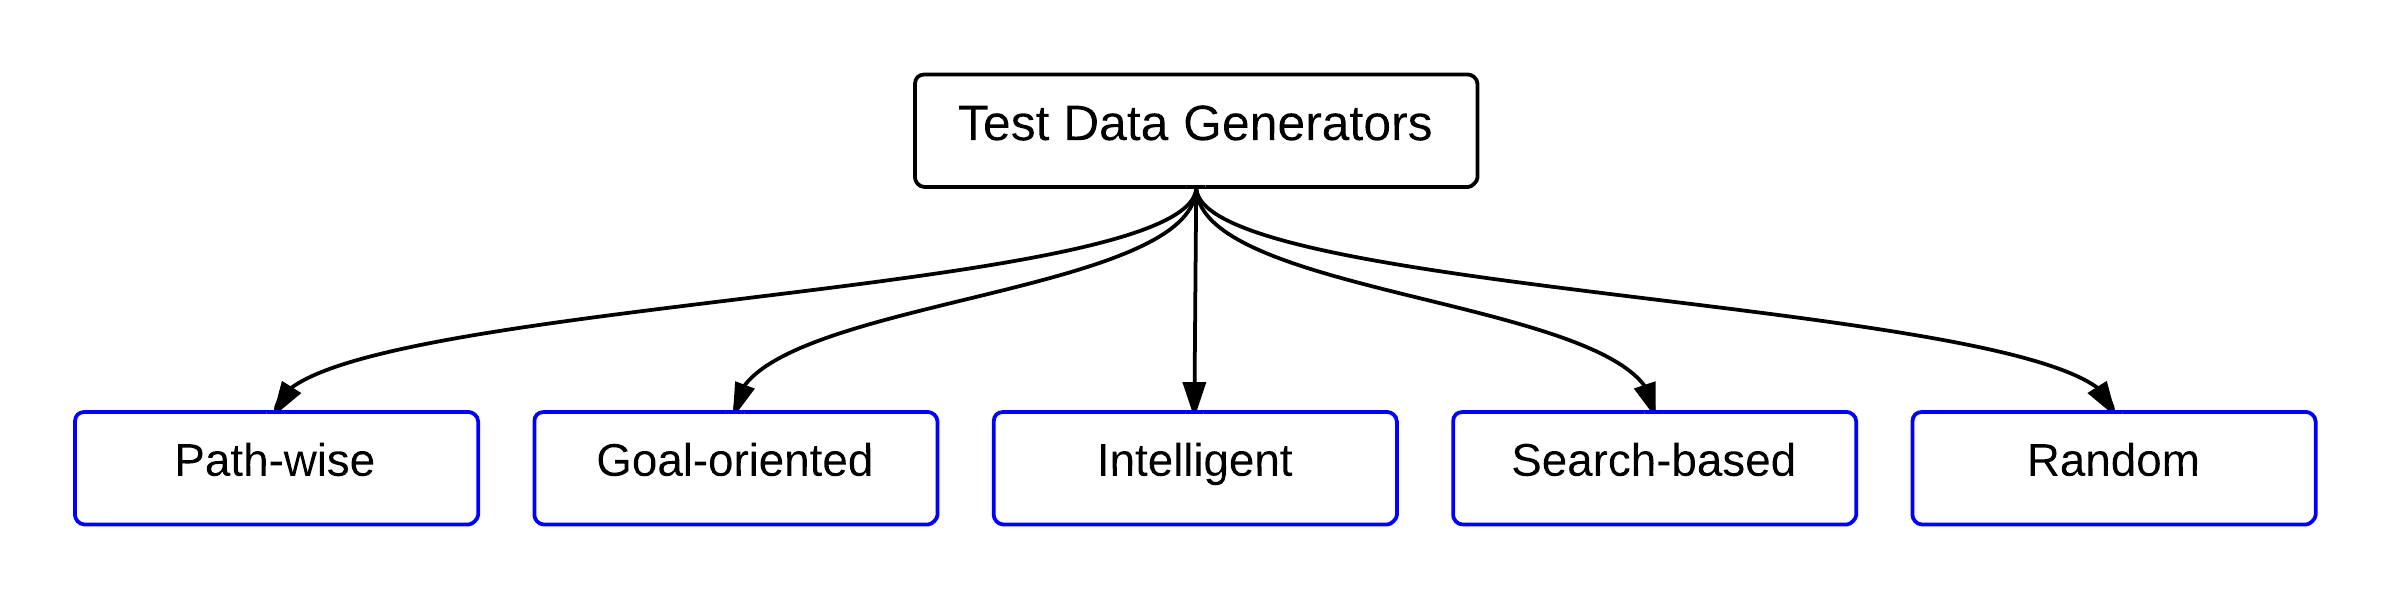
\includegraphics[width=16.5cm, height=5.2cm ]{chapter2/Generators.png}}
	\caption{Types of test data generator}
	\label{testDataGenerators_2}
\end{figure}

\subsection{Path-wise Test Data Generator} 
\label{sec:pathwise_2}
Path-wise test data generator generates data to target path, statement and branch coverage in a given SUT. The approach generally consists of three main parts: CFG construction, path selection and test data generation. 

In path-wise test data generation, the program path to the selected statement is identified and the input data are generated automatically or provided by the user for evaluating the path. The data generated in path testing expresses boolean behaviour i.e. true or false for a particular node in a path. A complete path contains multiple sub-domains, each sub-domain consists of test inputs required to traverse the path. The boundary of the sub-domains are obtained by the predicates in the path condition. The test data traversing a certain path in the software are selected from an input space split into a set of sub-sections. 

% the pathwise test data generation is taken from a book knowldge mining using intelligent systems. you can reference it too.


\subsection{Goal-oriented Test Data Generator}
\label{sec:goaloriented_2}
Goal-oriented test data generator generates data to target a specific program point rather than a program path \cite{chungautomated}. The tester can select any path among a set of existing paths as long as it reaches the specified program point. This technique utilizes runtime information for computing accurate test data~\cite{ferguson1996chaining}. Among various methods used in goal-oriented test data generation the following two commonly adopted approaches are briefly described.

\subsubsection{Chaining Approach}
The chaining approach uses data dependent analysis to guide the test data generation. In the process all the related statements affected by execution of the statement under test are selected automatically. The dependant statements are executed before the selected statement to generate the required necessary data for the execution of the statement under test~\cite{ferguson1996chaining}. The chaining approach analyses the program according to the edges and nodes. For each test coverage criterion different initial event sequence and goal nodes are determined. For example, consider  the branch (p, q), where p is  the starting node of the branch and q is the last node in the branch. The initial event sequence E for the branch (p, q) is defined as $E =< (s,\phi), (p,\phi),(q,\phi) >$, provided that s is the starting node of the program and $\phi$ is the set of variables referred to as constraint. The Branch classification process identifies critical, semi-critical and non-critical nodes for each branch. During execution, the classification guides the search process to select specific branches to reach the goal node.  

\subsubsection{Assertion-oriented Approach}
The assertion-oriented approach adds assertions to the program code with the goal to identify program input on which an assertion is violated indicating a fault in the SUT. An assertion is a constraint applicable to a state of computation which can be either true or false. For example, consider a given assertion A, now find program input x on which assertion A is false, i.e. when the program is executed on input x and the execution reaches assertion A, it is evaluated as false indicating a fault in the SUT. It is not always possible to generate test cases that violate assertions. However, experiments have shown that assertion-oriented test data generation may frequently detect errors in the program related to assertion violation. The major advantage of this approach is that each generated test data uncovers an error in the program with violation of an assertion. An assertion is violated due to fault in program code, in pre or post-condition or a fault in the assertion itself.

% check the korel1996assertion for the above whole text and assertion oriented approach + the model hard copy thesis.


\subsection{Intelligent Test Data Generator}
\label{sec:intelligent_2}
The intelligent test data generator is used to overcome the problems associated with traditional data generators like generation of meaningless data, duplicated data and complex data. The approach increases users confidence in the generated test data and the testing process~\cite{ramamoorthy1975testing}. It helps in finding the appropriate test data by performing sophisticated analysis to anticipate different situations that may arise at any point in the SUT, such as fuzzy logic, neural network and genetic algorithm. The approach produces test data which satisfy the SUT requirements but consumes more time and resources.

\subsubsection{Genetic Algorithm}
Genetic algorithm is a heuristic that mimics the evolution of natural species for searching optimal solution of a problem. The genetic algorithm is guided by control dependencies in the program to search for data which satisfy test requirements. The algorithm evaluates the existing test data, and guide the direction of search by using the program control-dependence graph \cite{pargas1999test}. The approach emphasises on the execution of a given statement, branch, path and condition in the given SUT. The benefit of the genetic approach is quick generation of test cases with proper focus and direction. The new test cases are generated by applying simple operations on the appropriate existing test cases having good potential of satisfying the test requirements. The success of the approach depends heavily on the way in which the existing test data are measured \cite{pargas1999test}.

% Please paraphrase the above section genetic algorithm.

\subsection{Search-based Test Data Generator} \label{sec:search_based_2}
Search-based test data generator uses meta-heuristic algorithms to generate test data. In this technique each input vector~\verb+x+ can be associated with a measure ~\verb+cost(x)+ which represents the difference between the input value~\verb+x+ and the set goal. Input value closer to the set goal has low cost value as against the input value away from the set goal. \\*
Let us consider the following program.


\begin{lstlisting}
void test(int x,int y) {
	if (x >= 20) {
		y = z; 
	}
	else {
		y = 2 * z;
	}
}
\end{lstlisting}

Suppose we want the true branch of the if/else statement to be executed. An input value of~\verb+x == 25+ clearly satisfies the predicate, and a value of~\verb+x == 15+ can be seen to come closer to satisfying the predicate than a value of~\verb+x ==5+. We might evaluate a cost function probe of the form~\verb+cost(x) = max {0, 20 - x}+. Thus \verb+x == 25+ has cost~\verb+0+,~\verb+x == 15+ has cost~\verb+5+ and~\verb+x = 5+ has cost~\verb+15+. It is apparent that finding data to satisfy the branch predicate is essentially a search over the input domain of ~\verb+x+ to find a value such that~\verb+cost(x) == 0+. The data which satisfy each of the predicates at different points may be selected to follow a particular path in the code. This leads to a cost function which combines costs at each of the relevant branching point. The cost function plays the role of oracle for each targeted test requirement. Consequently, the cost function must change as per requirement. Frequent re-instrumentation of program is required to find test data that fully satisfy common coverage criteria. 

%the cost function plays the role of oracle for each targeted test requirement.
%At its heart search based software testing requires the use of search or optimisation algorithms. Most standard heuristic search techniques have been used, e.g. hill-climbing, simulated annealing, tabu search and genetic algorithms. 

% The details need not concern us here, and the reader is referred to McMinn [50] for details. Overall the search based 





%\subsection{Using A Model Checker}
%\subsection{Test Case Generation with Gatel by Using Lustre}
%\subsection{Using Models in Z}
%\subsectioin{Using UML Diagrams}
%\subsection{Using Misuse / Abuse Cases for Robustness Testing}
%\subsection{Randomly-generated test suites} % Dynamically discovering likely program invariants thesis page 77
%\subsection{Grammar-generated test suites Randomly}% Dynamically discovering likely program invariants thesis page 78
%\subsection{Test-case generation} %Combining over-and under-approximating program analysis for automatic software testing (section 4.2)
%\subsection{Mutation generation} % Automatic testing of software with structurally complex inputs. page 79 section 7.2.1
%\subsection{Test Data Generation} % page 70, 4.6.1, Coverage analysis for GUI Testing
% Check Generating Structurally complex tests from declarative constraints thesis 




% add diagram for generators similar to john paper in automated program flaw finding using simulated annealing.


\subsection{Random Test Data Generator}
\label{sec:randomgenerator_2}
Random test data generator is the simplest approach for generation of test data. Its advantage is the adaptability to generate input data for any type of program. However, random test data generation is based solely on probability and cannot accomplish high coverage as its chances of finding semantically small faults are quite low~\cite{godefroid2005dart}. If a fault is only revealed by a small percentage of the program input it is said to be a semantically small fault. As an example of a semantically small fault, consider the following code:

\begin{lstlisting}
void test(int x, int y) {
    if (x==y){
        System.out.println("Equal");
    }
    else {
        System.out.println("Not Equal");
    }
}
\end{lstlisting}

It is clear that the probability of execution of the first statement is significantly lower than that of the second statement. As the structure gets more and more complex, the probability of execution decreases accordingly. Thus semantically small faults are hardly detectable by using random test data generator. 



\section{Random Testing}
Random testing is mentioned in the literature for the first time by Hanford in 1970. He reported syntax machine, a tool that randomly generated data for testing PL/I compilers~\cite{hanford1970automatic}. Later in 1983, Bird and Munoz described a technique to produce randomly generated self checking test cases~\cite{bird1983automatic}. 

%Work on random test generation dates back to a 1970 paper by Hanford. In it he reports on the ``syntax machine", a program that generated random but syntactically-correct programs for testing PL/I compilers \cite{hanford1970automatic}. The next published work on random testing was a 1983 paper by Bird and Munoz \cite{bird1983automatic}. They describe a technique to generate randomly-generated ``self-checking" test cases: test cases that in addition to generating test inputs generated checks for expected outputs using knowledge of the semantics of the software under test. For example, when generating random programs for testing a compiler, the generator kept track of the expected values of arithmetic computations and inserted the appropriate checks into the test case. They also applied their technique to checking sorting and merging procedures and graphic display software~\cite{pacheco2009directed}.

%One of the best-known works in the field is Miller et al.’s “fuzz testing” paper, where they generate random ASCII character streams and use them as input to test Unix utilities for abnormal termination or non-terminating behaviour \cite{miller1990empirical}. In subsequent work, they extended fuzz testing to generate sequences of keyboard and mouse events, and found errors in applications running in X Windows, Windows NT and Mac OS X \cite{forrester2000empirical, miller2006empirical}. Today, fuzz testing is used routinely in industry. It is frequently used as a tool for finding security vulnerabilities and is applied to test formats and protocols that attackers might use to gain unauthorized access to computers over a network. Other work that applies random test generation to operating systems code includes Kropp’s use of random test generation to test low-level system calls \cite{kropp1998automated}, and Groce et al.’s use of random test generation at NASA to test a file system used in space missions \cite{groce2007randomized}. In all these studies, a random test generator invariable found many errors in the software under test, and many errors were critical in nature. For example, Groce et al. found dozens of errors in the file system under test, many of which could have jeopardized the success of a mission.

Random testing is a dynamic black-box testing technique in which the software is tested with non-correlated unpredictable test data from the specified input domain~\cite{chan2003normalized}. As stated by Richard~\cite{hamlet1994random}, input domain is first identified then test data are randomly taken from it by means of random generator. The program under test is executed on the test data and the results obtained are compared with the program specifications. The test fails if the results are not according to the specifications and vice versa. Fail results of the test cases reflects failure in the SUT. Working mechanism of random testing is shown in Figure \ref{fig:workingmechanism}.

%\begin{figure}[h]
%	\centering
%	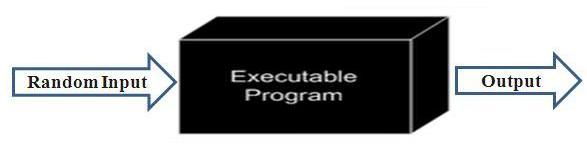
\includegraphics[width=11cm, height=2.5cm ]{chapter2/randomTesting.jpg}
%	\caption{Random Testing}
%\end{figure}



\begin{figure}[h]
	\centering
	\centerline{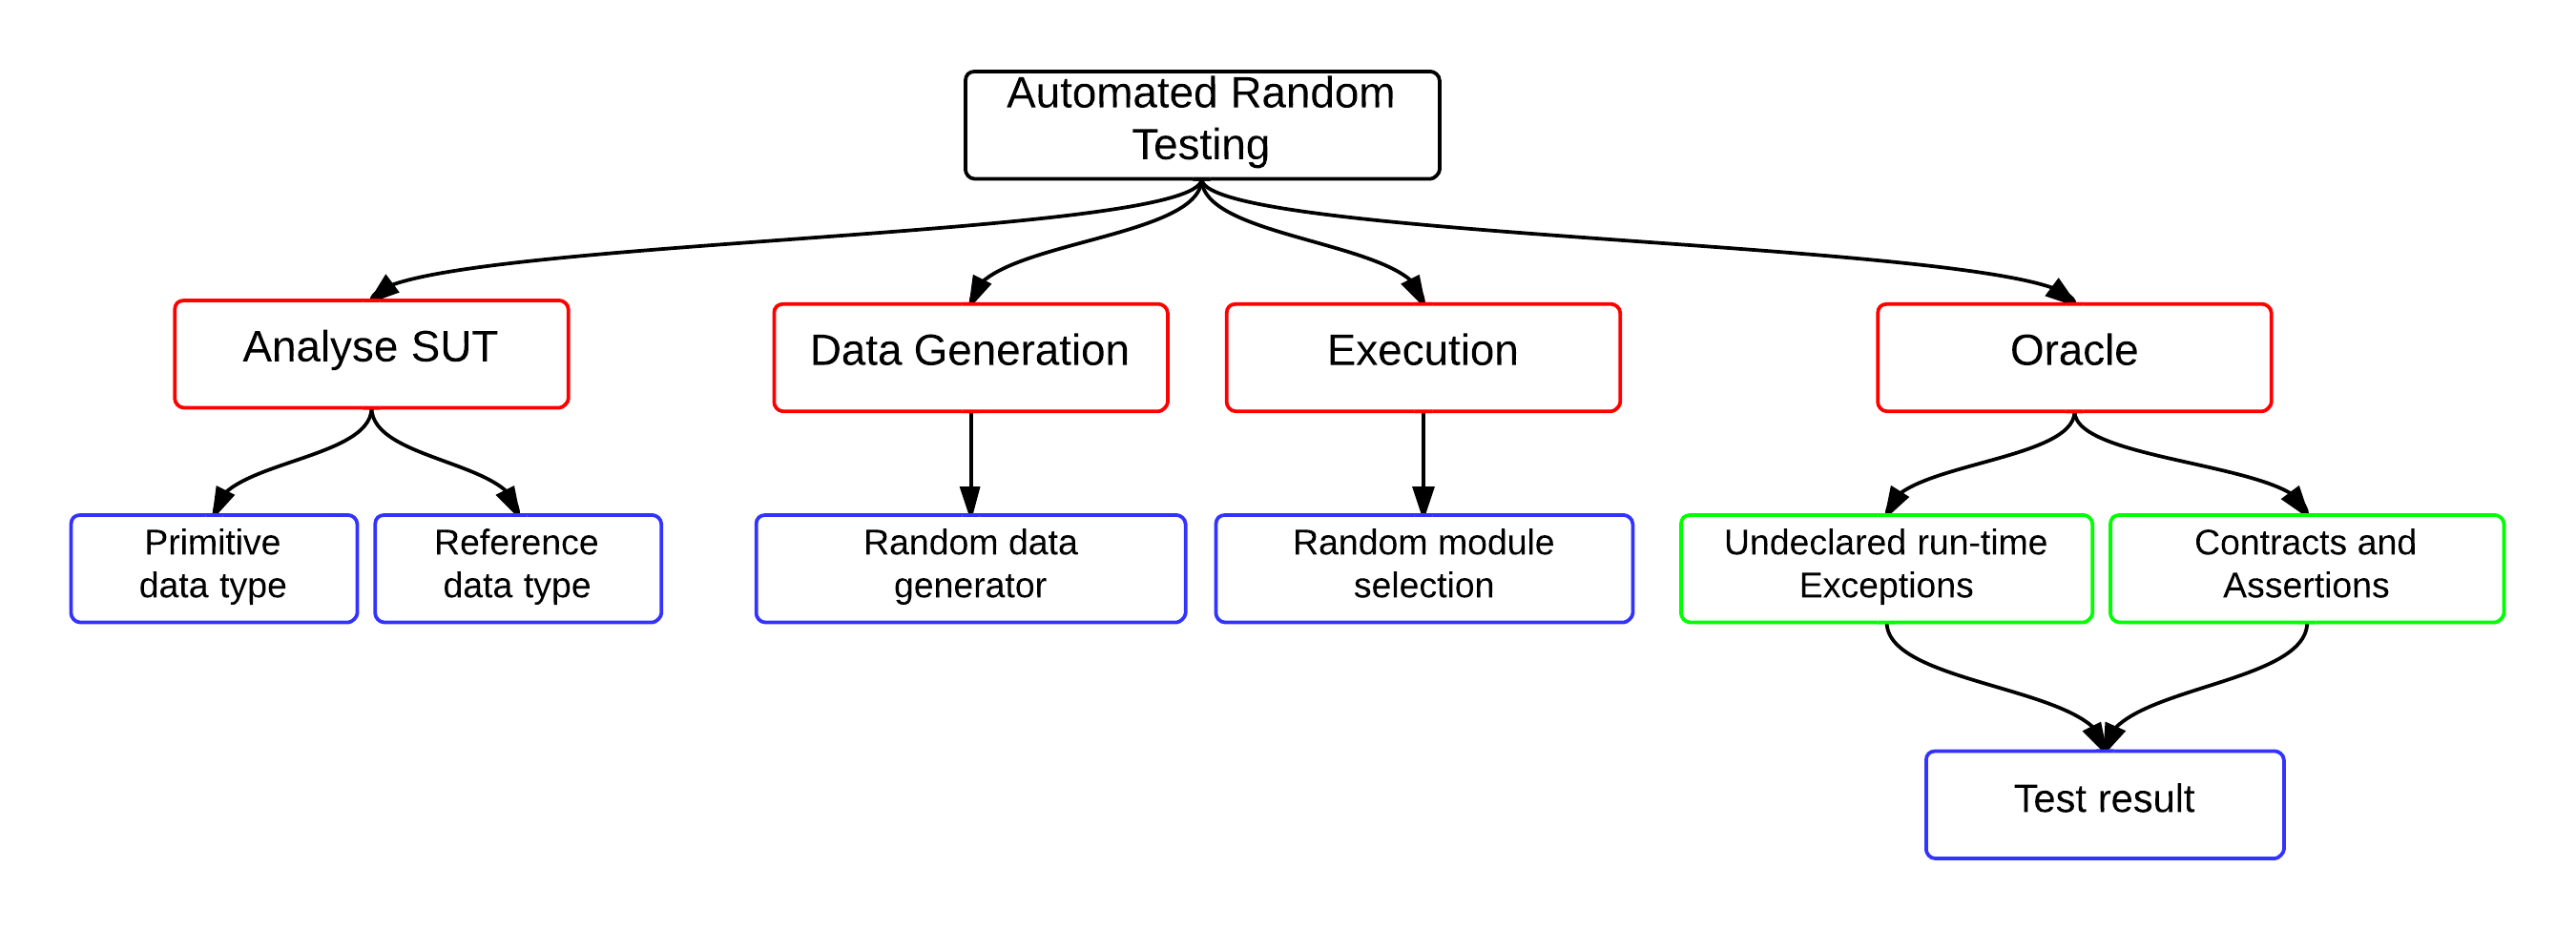
\includegraphics[width=16.5cm, height=9cm ]{chapter2/randomTestingMechanism.png}}
	\caption{Working mechanism of random testing}
	\label{fig:workingmechanism}
\end{figure}

Generating test data by random generator is economical and requires less intellectual and computational efforts~\cite{ciupa2008artoo}. Moreover, no human intervention is involved in data generation which ensures an unbiased testing process. However, generating test cases with out using any background information makes random testing susceptible to criticism. Random testing is criticized for generating many of the test cases that falls at the same state of software. It is also stated that, random testing generates test inputs that violates requirements of the given SUT making it less effective~\cite{pacheco2009directed, sen2007effective}. Myers mentioned random testing as one of the least effective testing technique~\cite{myers2011art}. However, Ciupa et al.~\cite{ciupa2007experimental} stated that Myers statement is not based on any experimental evidence. Later experiments performed by several researchers~\cite{ciupa2008finding, hamlet1994random,  leitner2007efficient} confirmed that random testing is as effective as any other testing technique. It is reported~\cite{duran1981report} that random testing can also discover subtle faults in a given SUT when subjected to large number of test cases. It is pointed out that the simplicity and cost effectiveness of random testing makes it more feasible to run large number of test cases as opposed to systematic testing techniques which require considerable time and resources for test case generation and execution. The empirical comparison shows that random testing and partition testing are equally effective~\cite{hamlet1990partition}. Ntafos~\cite{ntafos1998random} conducted a comparative study and concluded that random testing is more effective as compared to proportional partition testing. Miller et al.~\cite{miller1990empirical} generated random ASCII character streams and used the Unix utilities for abnormal terminating and non-terminating behaviours. Subsequently, the technique was extended to discover errors in software running on X Windows, Windows NT and Mac OS X~\cite{forrester2000empirical, miller2006empirical}. Other famous studies using random testing includes low-level system calls \cite{kropp1998automated} and file systems used in missions at NASA \cite{groce2007randomized}.






\section{Input Domain} 
The input domain comprises all possible inputs for a software, including all global variables, method arguments and externally assigned variables. For a given program P with input vector $ P =\{x1, x2, . . . , xn\}$, having $\{D1, D2, . . . , Dn\}$ as the domain of each input so that $x1 \in D1, x2 \in D2$ and so on, the domain D of a function is the cross product of the domains of each input: $D = D1 \times D2 \times . . . \times Dn$.

\subsection{Genuine and Failure-domain} \label{sec:failuredomains_2}
\label{sec:genuineandfailuredomain}
Chan et al. \cite{chan1996proportional} observed that input inducing failures are contiguous and form certain geometrical shapes in the whole input domain and divided these into point, block and strip failure-domains as described below.

\begin{enumerate}
\item {\bf Point:} In the point failure-domain, input inducing failures are scattered across the input domain in the form of stand-alone points. Example of point failure-domain is the failure caused by the statement: $total = num1/num2;$ where $num1$, $num2$ and $total$ are variables of type integer.
\item {\bf Block:} In the block failure-domain, input inducing failures lie in close vicinity to form a block in the input domain. Example of block failure-domain is failure caused by the statement: $if ( (num \textgreater 10) \&\& (num \textless 20) )$. Here 11 to 19 are a block of failures.
\item {\bf Strip:} In the strip failure-domain, input inducing failures form a strip across the input domain. Example of strip failure-domain is failure caused by the statement: $num1 + num2 = 20$. Here multiple values of $num1$ and $num2$ can lead to the fault value 20. 
\end{enumerate}

\begin{figure} [H]
\centering
\subfigure[Point domain]{
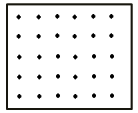
\includegraphics[width=3.6cm,height=3.6cm]{chapter2/point.png}
\label{fig:point}
}
\subfigure[Block domain]{
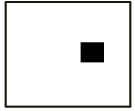
\includegraphics[width=3.6cm,height=3.6cm]{chapter2/block.png}
\label{fig:block}
}
\subfigure[Strip domain]{
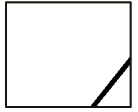
\includegraphics[width=3.6cm,height=3.6cm]{chapter2/strip.png}
\label{fig:strip}
}

\caption{Failure domains across input domain~\cite{chan1996proportional}}
\label{fig:patterns2}
\end{figure}


%\begin{figure}[h]
%	\centering
%	\centerline{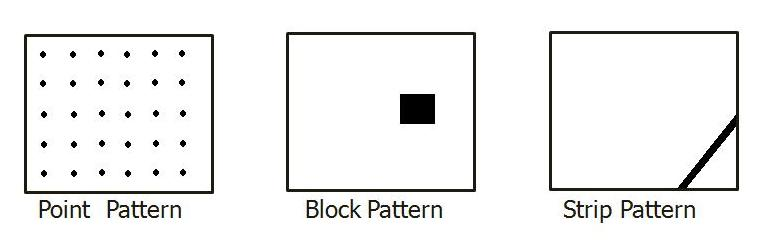
\includegraphics[width=13cm, height=5cm ]{chapter2/pointblockstrip.jpg}}
%	\caption{Domains of failure causing inputs~\cite{chan1996proportional}}
%	\label{fig:patterns2}
%\end{figure}

Figure~\ref{fig:patterns2} shows failure domains across the input domains. The square boxes in the figure indicate the whole input domain, the white space in each box shows legitimate and faultless values while the black colour in the form of points, block and strip indicate failures in the form of point, block and strip failure-domains.

\newpage
\section{Versions of Random testing}
Researchers have tried various approaches to develop new versions of random testing for better performance. The prominent improved versions of random testing are shown in Figure \ref{fig:randomTestingVersions_2}.
\begin{figure}[H]
	\centering
	\centerline{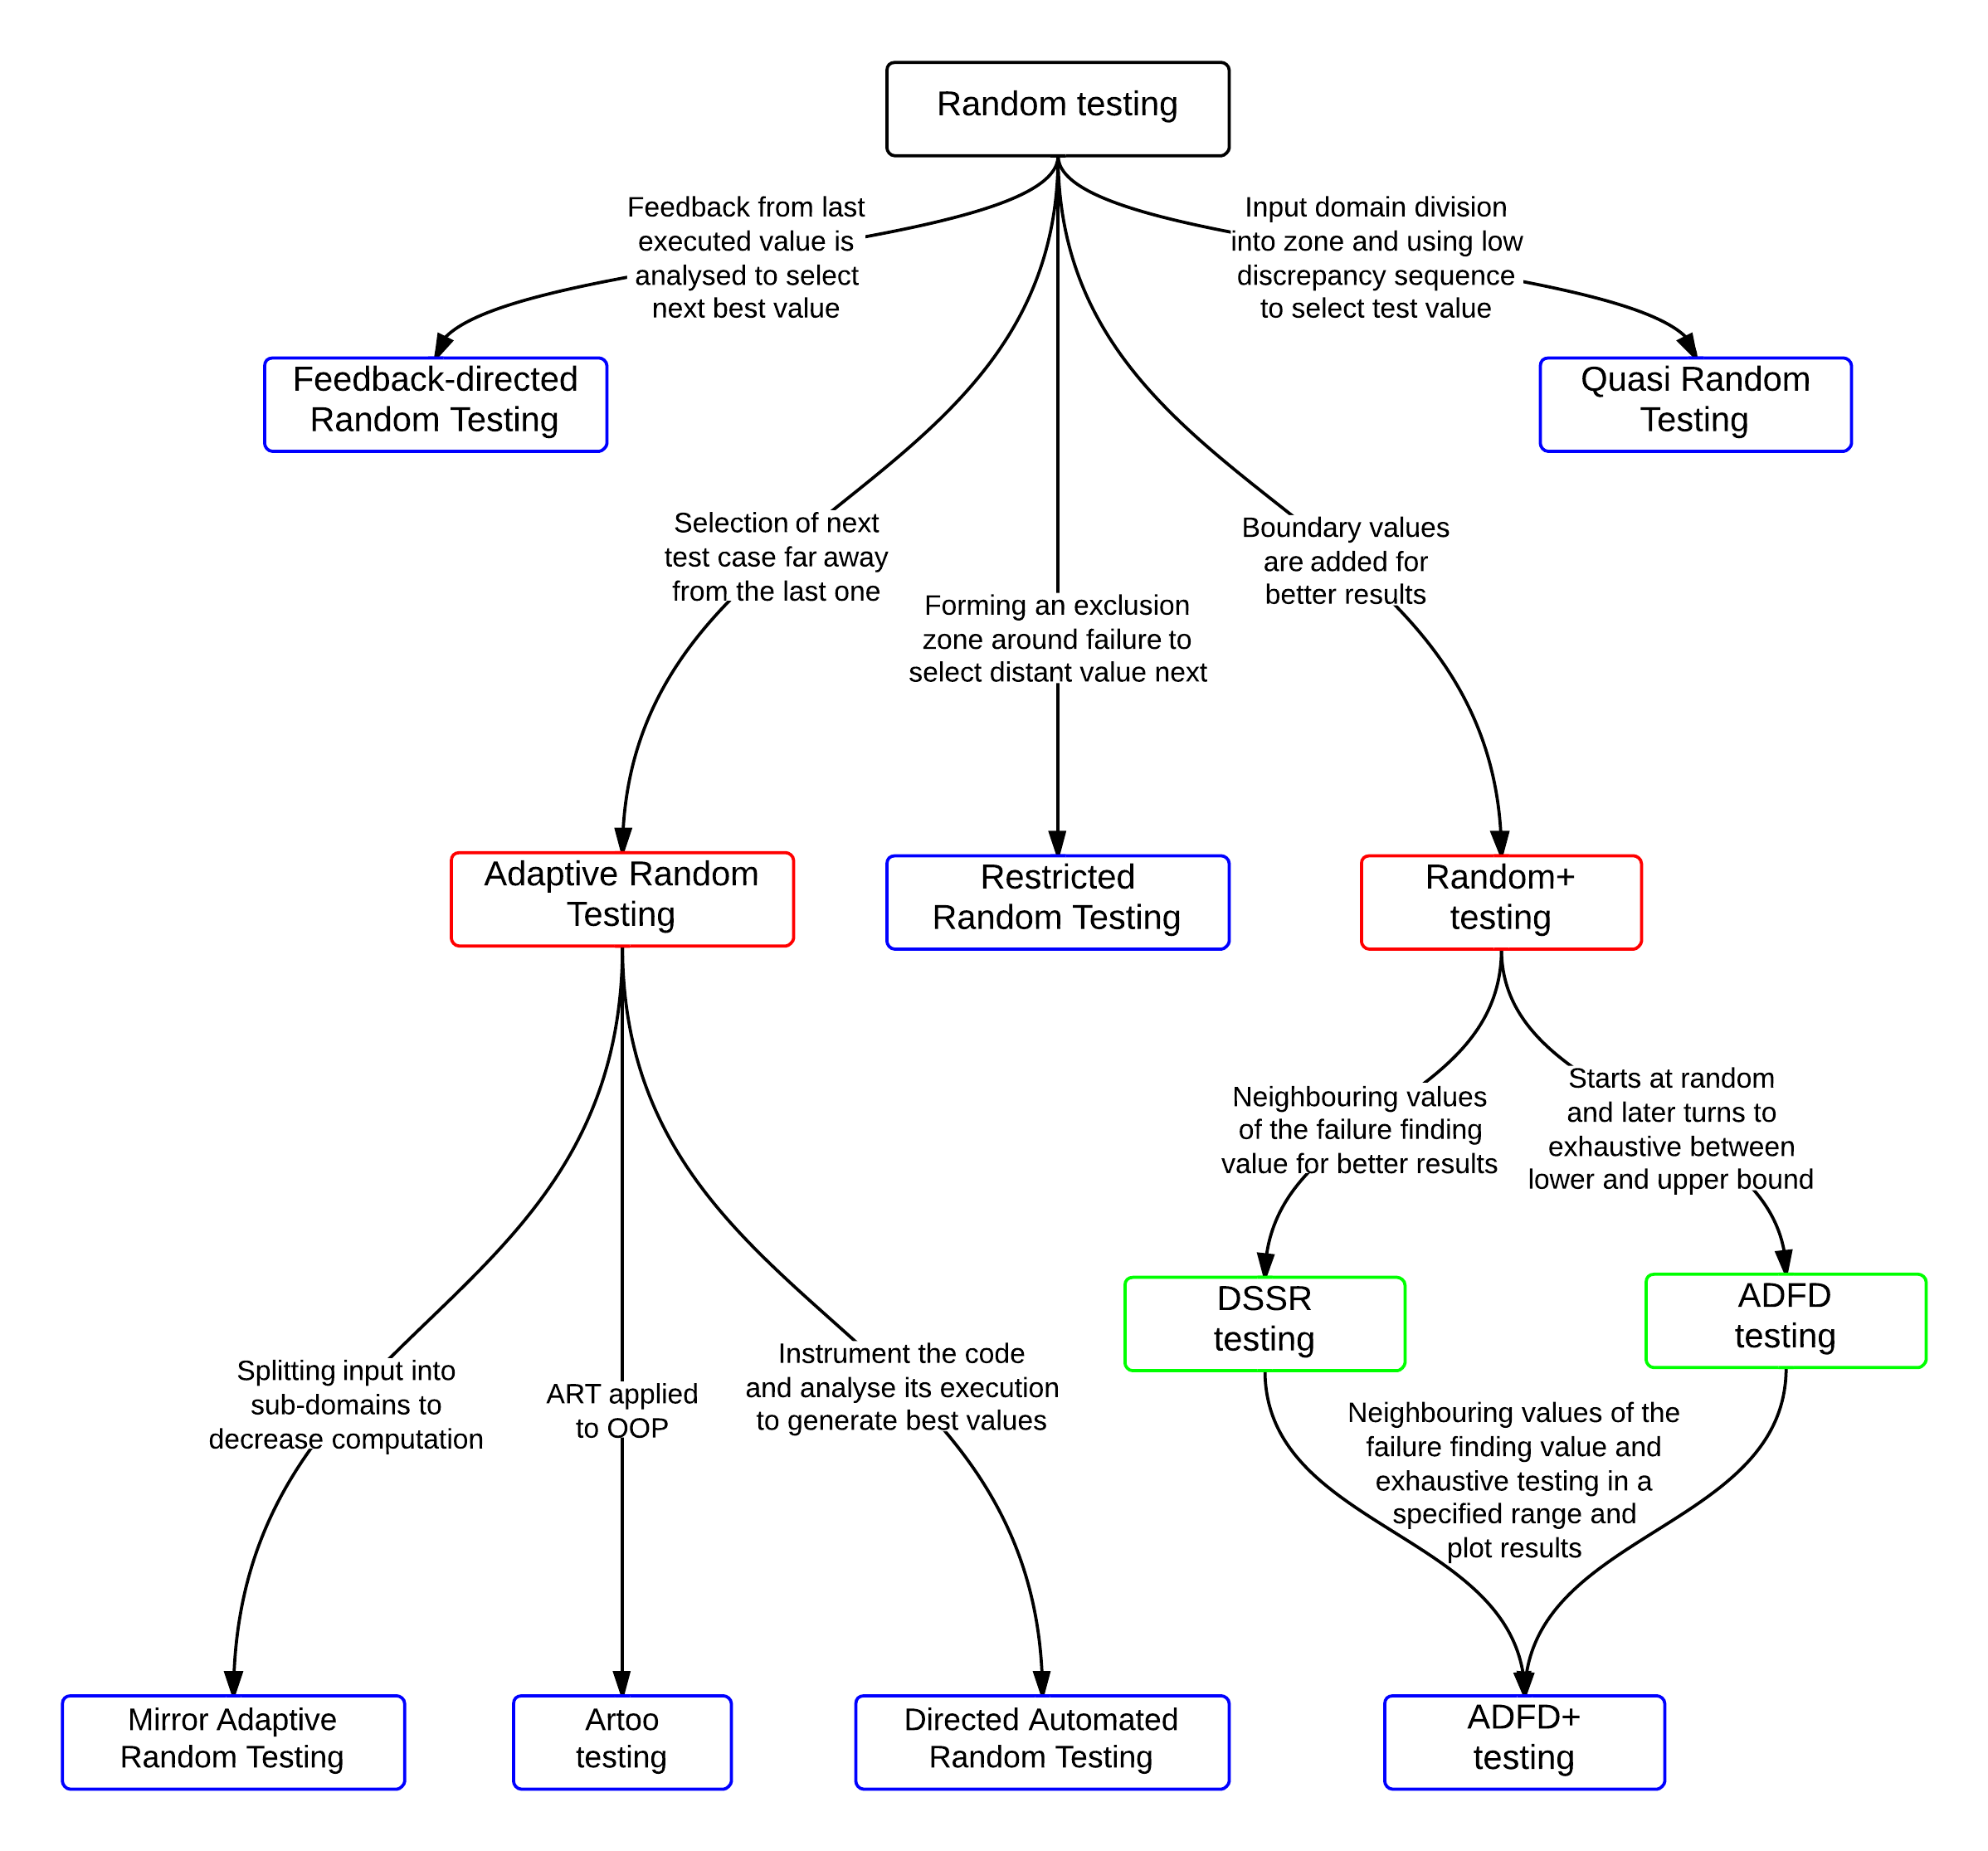
\includegraphics[width=16.5cm, height=18cm]{chapter2/randomTestingVariations.png}}
	%\centerline{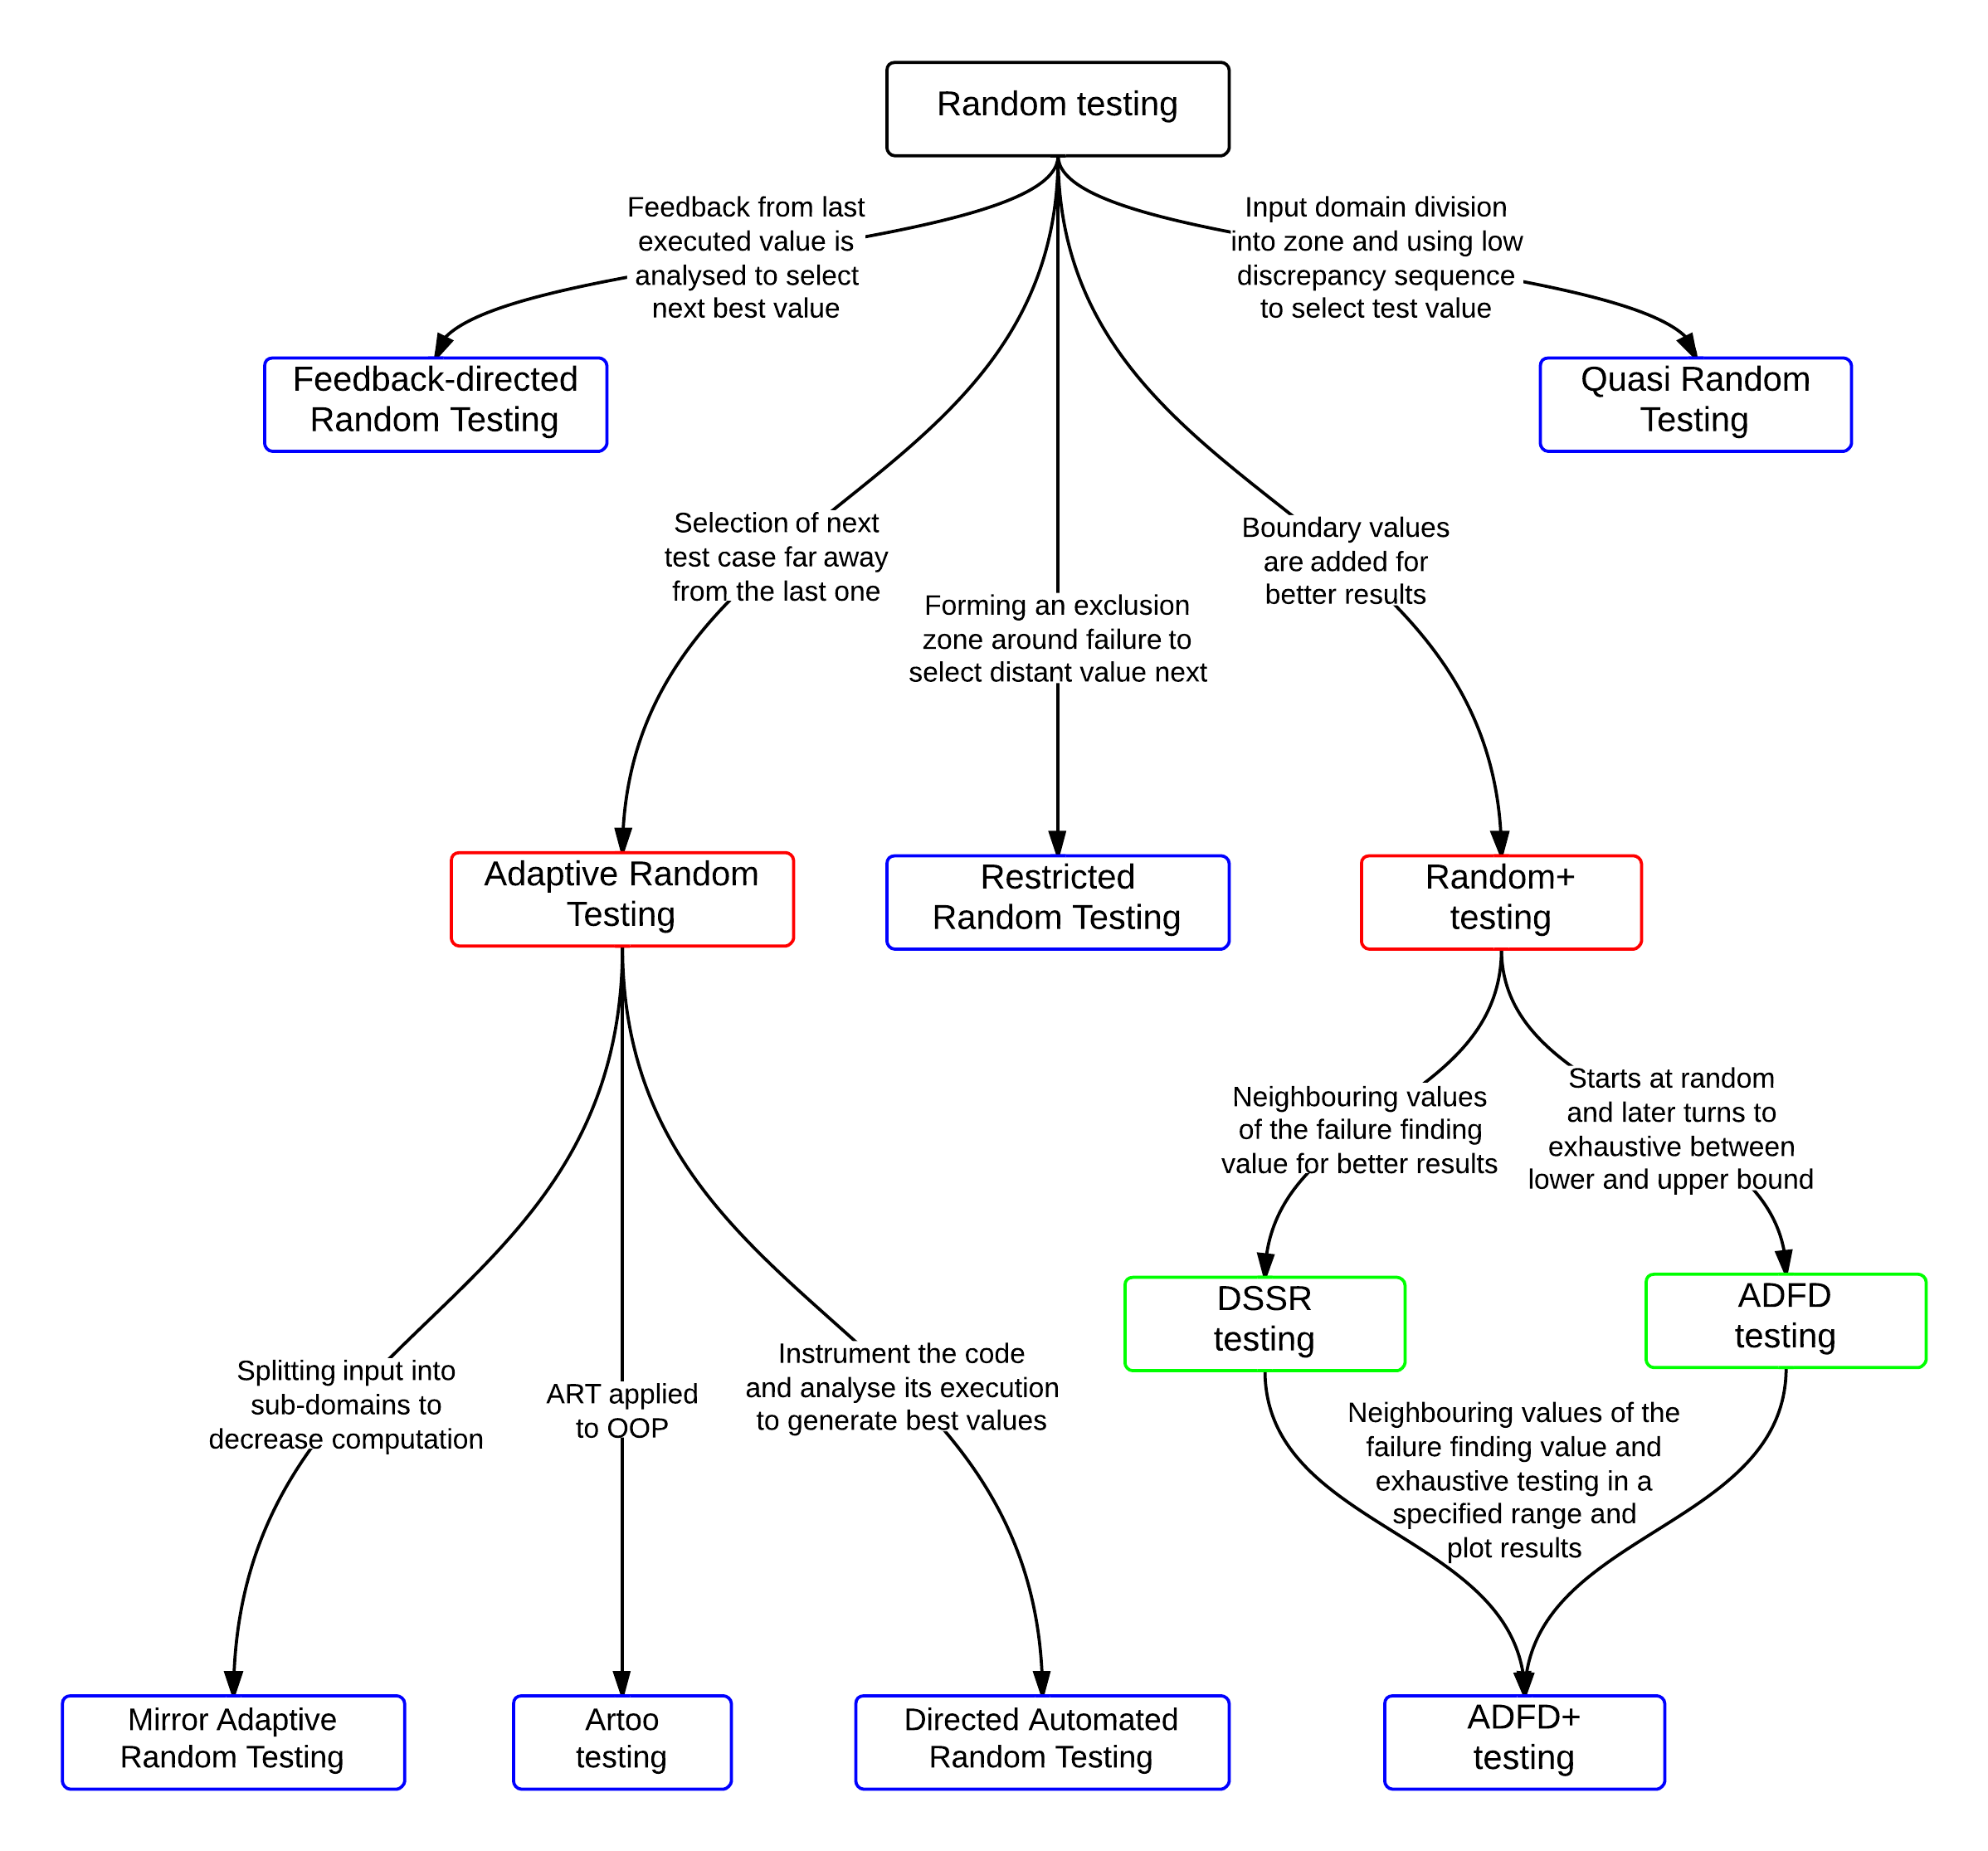
\includegraphics[width=\textwidth]{chapter2/randomTestingVariations.png}}
	\caption{Various versions of random testing}
	\label{fig:randomTestingVersions_2}
\end{figure}

\subsection{Random+ Testing}
The random+ testing~\cite{leitner2007reconciling} is an extension of the random testing. It uses some special pre-defined values which can be simple boundary values or values that have high tendency of finding faults in the SUT. Boundary values~\cite{beizer2003software} are the values at the start and end of a particular data type. For instance, such values for \verb+int+ could be \verb+Integer.MAX_VALUE+, \verb+Integer.MAX_VALUE-1+, \verb+Integer.MAX_VALUE-2+; \verb+Integer.MIN_VALUE+, \verb-Integer.MIN_VALUE+1-, \verb-Integer.MIN_VALUE+2-. These special values can add a significant improvement to a testing method. \\*
Let us consider the following piece of code:

\begin{lstlisting}
public void test (int arg) {
	arg = arg + 1;
	int [] intArray = new intArray[arg];
	...
}
\end{lstlisting}

In the given code, on passing interesting value \verb+MAX_INT+ as argument, the code increment it by 1 making it a negative value and thus an error is generated when the system tries to build an array of negative size. Similarly, the tester might add some other special values that he considers effective for finding faults in the SUT. For example, if a program under test has a loop from -50 to 50 then the tester can add -55 to -45, -5 to 5 and 45 to 55 to the pre-defined list of special values. This static list of interesting values is manually updated before the start of the test. Interesting values included in the list is given slightly higher priority than random values because of their relevance and better chances of finding faults in the given SUT. As reported in the literature, The interesting values have high impact on the results, particularly for detecting problems in specifications~\cite{ciupa2008finding}.


\subsection{Adaptive Random Testing}
\label{sec:artpatterns_2}
Adaptive random testing (ART) proposed by Chen et al.~\cite{chen2005adaptive} is based on the previous work of Chan et al.~\cite{chan1996proportional} regarding the existence of failure domains across the input domain (Section~\ref{sec:genuineandfailuredomain}). Chen et al.~\cite{chen2005adaptive} argued that ordinary random testing might generate test inputs lurking too close or too far from the input inducing failure and thus fails to discover the fault. To generate more fault-targeted test inputs, they proposed Adaptive Random Testing (ART) as a modified version of random testing where test values are selected at random as usual but are evenly spread across the input domain by using the executed set and the candidate set. Initially both sets are empty but as soon as the testing begins ART technique populates the candidate set with randomly selected test cases from the input domain. The first test case selected at random from the candidate set is executed and then stored in the executed set. The second test case is the one selected from the candidate set which is located far away from the previous executed test case. The process continues till test completion resulting in greater chances of finding failures from failure domains.

Chen et al.~\cite{chen2005adaptive} used ART in their experiments with the number of test cases required to detect first fault (F-measure) as a performance matrix instead of the traditional matrices (P-measure) and (E-measure). The results showed up to 50\% increase in performance compared to random testing. However, the authors pointed out issues of spreading test cases across the input domain for complex objects, efficient ways of selecting candidate test cases and higher overhead are yet to be resolved. Chen et al.~\cite{chen2009enhanced} continued their work on ART for addressing the issues and proposed the following upgraded versions. 

\subsection{Mirror Adaptive Random Testing}
%As discussed in the above section ART provide better results, however the increase in overhead due to extra computation to achieve even spread of test inputs makes it less cost effective. 
Mirror Adaptive Random Testing (MART) is an improvement on ART by using mirror-partitioning technique to reduce the overhead by decreasing the extra computation involved in ART~\cite{chen2004mirror}. 

\begin{figure}[h]
\begin{center}
	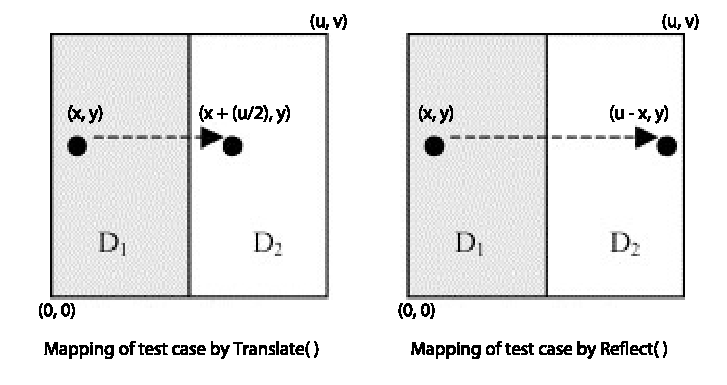
\includegraphics[width=13.5cm, height=6.5cm ]{chapter2/mart2.pdf}
	\caption{Mirror functions for mapping of test cases}
\label{fig:mirrorART}
\end{center}  
\end{figure}

In this technique, the input domain of the program under test is divided into n number of disjoint sub-domains of equal size and shape. One of the sub-domains is called source sub-domain while all others are termed as mirror sub-domains. ART is then applied only to the source sub-domain while test cases are selected from all other sub-domains by using mirror function. In MART \verb+(0, 0), (u, v)+ are used to represent the whole input domain where \verb+(0, 0)+ is the leftmost and \verb+(u, v)+ is the rightmost top corner of the two dimensional rectangle. On splitting it into two sub-domains we get \verb+(0, 0), (u/2, v)+ as source sub-domain and \verb+(u/2, 0), (u, v)+ as mirror sub-domain. Suppose we get \verb+x+ and \verb+y+ test cases by applying ART to source sub-domain, so we can linearly translate these test cases to achieve the mirrored effect, i.e. \verb+(x + (u/2), y)+ as shown in Figure~\ref{fig:mirrorART}. Comparative study of MART with ART provides evidence of equally good results of the two strategies with MART having the added advantage of lower overhead by using only one quarter of the calculation as compared with ART.


\subsection{Restricted Random Testing}
Restricted Random Testing (RRT) is another approach~\cite{chan2003normalized} to overcome the problem of extra overhead in ART. The RRT achieves this by creating a circular exclusion zone around the executed test case. A candidate is randomly selected from the input domain for the next test case. Before execution the candidate is checked and discarded if it lies inside the exclusion zone. This process repeats until a candidate present outside the exclusion zone is selected. It ensures that the test case to be executed is well apart from the last executed test case. The radius of exclusion zone is constant in each test case and the area of input domain decreases progressively with successive execution of test cases.

\begin{figure}[h]
	\centering
	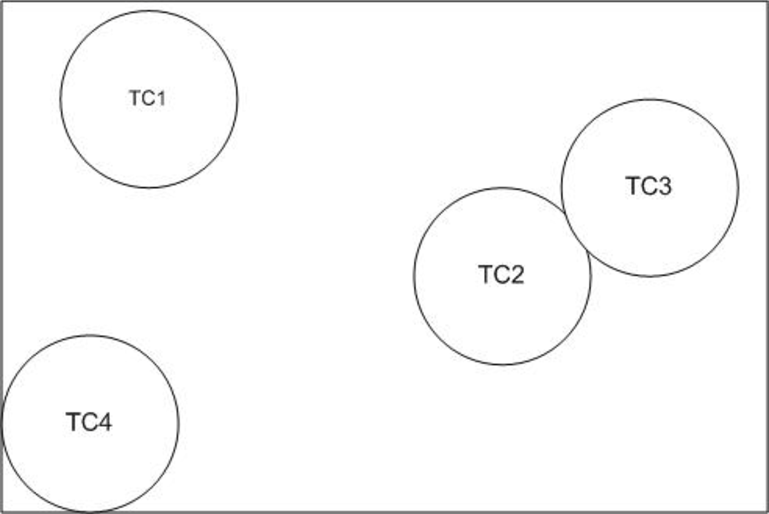
\includegraphics[width= 8cm, height = 6.5cm]{chapter2/RRT.pdf}
	\caption{Input domain showing exclusion zones around selected test cases}
\end{figure}

The authors~\cite{chan2003normalized} compared RRT with ART and RT to find the comparative performance and reported that the performance of RRT increases with the increase in the size of the exclusion zone and reaches the maximum level when the exclusion zone is raised to the largest possible size. %Normalized Restricted Random Testing~\cite{chan2003normalized} is an improvement over RRT by allowing the testers to have better information about the target exclusion rate (R) of RRT. 
They further found that RRT is up to 55\% more effective than random testing in terms of F-measure.



\subsection{Directed Automated Random Testing}
Godefroid et al.~\cite{godefroid2005dart} proposed Directed Automated Random Testing (DART). %Its main purpose was to overcome the cost and difficulty of manual testing while keeping its quality intact. It automate the whole testing process including generation of unit tests, test drivers/harness and assertions for functional correctness. 
The following main features of DART are reported in the literature:
\begin{enumerate}
\item {\bf Automated Interface Extraction:} DART automatically identifies external interfaces of a given SUT. These interfaces include external variables, external methods and the user-specified main method responsible for program execution.
\item {\bf Automatic Test Driver:} DART automatically generate test drivers for running the test cases. All the test cases are randomly generated according to the underlying environment.
\item {\bf Dynamic Analysis of execution:} DART instruments the given SUT at the start of the process in order to track its behaviour dynamically at run time. The results obtained are analysed in real time to systematically direct the test case execution along alternative path for maximum code coverage.
\end{enumerate}

The DART algorithm is implemented in the tool which is completely automatic and accepts the test program as input. After the external interfaces are extracted it uses the pre-conditions and post-conditions of the program under test to validate the test inputs. For languages that do not support contracts inside the code (like C), public methods or interfaces are used to mimic the scenario. DART attempts to cover different paths of the program code to trigger errors. Its oracle consists of checking for crashes, failed assertions and non-termination.



\subsection{Quasi Random Testing}
Quasi-random testing (QRT) is a testing technique~\cite{chen2007quasi} which takes advantage of failure region contiguity for distributing test cases evenly and thus decreases computation. %Chan et al after the analysis of faults in various experiments found that the fault patterns across the input domain are continuous. 
To achieve even spreading of test cases, QRT uses a class with a formula that forms an s-dimensional cube in s-dimensional input domain and generates a set of numbers with small discrepancy and low dispersion. The set of numbers is then used to generate random test cases that are per-mutatedf to make them less clustered and more evenly distributed. An empirical study was conducted to compare the effectiveness of QRT with ART and RT. The results showed that in 9 out of 12 programs QRT found a fault quicker than ART and RT while there was no significant improvement in the remaining three programs.
%\subsection{Monti Carlo Random Testing}

%\subsection{Good Random Testing}

\subsection{Feedback-directed Random Testing}
Feedback-directed Random Testing (FDRT) is a technique that generates unit test suite at random for object-oriented programs~\cite{pacheco2007randoop}. As the name implies FDRT uses the feedback received from the execution of first batch of randomly selected unit test suites to generate next batch of directed unit test suite. In this way redundant  and wrong unit tests are eliminated incrementally from the test suite with the help of filtration and application of contracts. For example if a unit test produces IllegalArgumentException on execution, it is discarded because the arguments used in the unit test is not according to the required type. 

%\subsection{Adaptive Random Testing for Object-Oriented}
\subsection{The Artoo Testing}
The Adaptive random testing for object oriented (Artoo) strategy is based on object distance. Ciupa et al.~\cite{ciupa2006object} defined the parameters that can be used to calculate distance between the objects. Two objects have more distance between them if they have more dissimilar properties. The parameters to specify the distance between the objects are dynamic types and values are assigned to the primitive and reference fields. Strings are treated in terms of directly usable values and Levenshtein formula~\cite{levenshtein1966binary} is used as a distance criterion between the two strings.

In the Artoo strategy, two sets are taken i.e. candidate-set containing the objects ready to be run by the system and the used-set which is initially empty. First object is selected randomly from the candidate-set which is moved to used-set after execution. The second object selected from the candidate-set for execution is the one with the largest distance from the last executed object present in the used-set. The process continues till the bug is found or the objects in the candidate-set are finished~\cite{ciupa2006object}.

The Artoo strategy, implemented in AutoTest~\cite{ciupa2008artoo}, was evaluated in comparison with Directed Random (D-RAN) strategy by selecting classes from EiffelBase library \cite{meyer1987eiffel}. The experimental results indicated that some bugs found by the Artoo were not identified by the D-RAN strategy. Moreover the Artoo found first bug with small number of test cases than the D-RAN strategy. However, more computation was required to select a test case in the Artoo strategy and the process took more time and cost to generate test cases as compared to D-RAN strategy.

% the same team implemented that model and performed several experiments to evaluate the proposed model. Adaptive Random Testing for Object Oriented (ARTOO) is a testing strategy, based on object distance, implemented in AutoTest \cite{16 search it Mendeley}.
%ARTOO was implemented as a plug-in strategy in AutoTest. It only deals with creating and selecting inputs and all other functionality of the AutoTest was the same. Since ARTOO is based on object distance therefore the method for test input selection is to pick that object from the candidate set (A pool of objects that is a potential candidate to be executed by the system) that has the highest average distance in comparison to the objects already executed. In the experiments classes from EiffelBase library \cite{17 search it mendeley} were used. To evaluate ARTOO the same tests were also applied to directed random strategy (RAND). The outcome of the experiments showed that ARTOO finds the first bug with fewer test cases than RAND. The computation to select test case in ARTOO is more than RAND and therefore ARTOO takes more time to generate a test input. The experiments also found few of the bug found by ARTOO were not pointed out by RAND furthermore ARTOO is less sensitive to the variation of seed value than RAND
. 
%\subsection{Object Distance and its application}
%To improve the performance of random testing the emphasis of ART was on the distance be- tween the test cases. But this distance was defined only for primitive data types like integers and other elementary input. Ciupa et al defined the parameters that can be used to calculate distance between the composite programmer-defined types so that ART can be applicable to testing of today’s object-oriented programs~\cite{Ciupa2006}. Two objects have more distance between them if they have more dissimilar properties. The parameters to specify the distance between the objects are dynamic types, values of its primitive and reference fields. Strings are treated as a directly usable values and Levenshtein distance~\cite{Levenshtein1966} that is also known as edit distance is used as a distance criteria between the two strings. To implement object distance first all the distances of the objects are measured. Then two sets candidate- objects containing the all the objects ready to be run by the system and the used-objects set, which is initially empty. First object is selected randomly from the candidate-object set and is moved to used-object set when executed by the system. Now the second object selected from the candidate set for execution is the one with the biggest distance from the last executed object present in the used-object set. This process is continuing until the bug is found or the objects in the candidate-object set are finished.

%\subsubsection{Experimental Assessment of RT for Object-Oriented Software}
%In this research the effect of various parameters involved in random testing and its effect on efficiency is evaluated by performing various experiments on Industrial-grade code base. Large-scale clusters of computers were used for 1500 hours of CPU time which resulted in 1875 test sessions for 8 classes under test.~\cite{Ciupa2007} The finding of the experiments are 1. Version of random testing algorithm that is efficient for smaller testing timeout is equally efficient for higher testing timeouts. 2. The value of seed for random testing algorithm plays a vital role in finding the number of bugs in specific time. 3. Most of the bugs are found in the first few minutes of the testing sessions.



%\subsection{Design by Contract}
% section taken from binding yeti with .net, check it out correct it.
%\textcolor{blue}{Modern software development as it is well known has adopted the paradigm of Object Oriented (OO) Programming. The primary and most important reason for this evolution is the desire for better quality software and a more efficient way to bridge the gap between requirements and code.
%Industrial use of OO confirmed the superiority of this approach over procedural
%programming languages. However, so far no final approach has been generally accepted over a methodology on how to construct OO software in order to achieve one of the most important factors of quality, which is reliability or else robustness. As the work of Dr. Bertrand Meyer has shown \cite{meyer1992applying, meyer1988object} the decision on how to make software more reliable is crucial if the developers want to use the benefits of OO. These benefits include:
%1 Reuse of software components. This implies using a software component at multiple environments apart from the environment in which its developers originally deployed it.
%2 The goal of having reliability plays an important role in characterizing the quality of a software module.
%3 The abstract types that OO introduces. A reliable way to construct abstract types emerges. To achieve the previous goals the software development world has used two approaches, Defensive programming and Design by Contract. As the next paragraphs show the latter one has been showing more advantages than the first one. That is why most researches on Automated Testing use design by contract as a requirement that the SUT must conform to, in order for their tool to find as many bugs as possible \cite{Leitner2007}.
%The idea of Defensive Programming, which is inherited from the software development world prior to OO, is in general advising to ―… include as many checks as possible even if they are redundant \cite{meyer1992applying}. This concept is intuitively stating that having extra checking can never do harm especially if someone wants to protect the software from inexperienced users. This last concept unfortunately is not correct. This kind of approach puts more code inside the software and this contributes to greater complexity of the software, and complexity as Dr. Meyer has very correctly stated ―…is the single worst obstacle to software quality in general, and to reliability in particular \cite{meyer1992applying}. The reason is that this extra code is a source of things that might go wrong and so we must also check it, and so on to infinitum. The need for a more systematic approach is evident based on the concept that software elements are implementations of well-understood specifications by the developers and that is exactly what Design by Contract does. Design by Contract concept adopts the idea that any operation a routine of a software performs, should bind the caller of that routine to the routine itself. This binding provides specific obligations that each party has, along with benefits. Essentially the obligations of one part describe the benefits of the other part. These ideas apply to software routines (i.e. methods, functions of classes) via assertions that implement the binding, which is like a contract between two persons. These assertions are classified into pre-conditions, post-conditions and class invariants. Figure 2.1 which is a figure of the ―Applying Design by Contract article \cite{meyer1992applying}, illustrates the use of these assertions.
%As anyone can understand from Figure ?? pre and post-conditions denote the idea that if the caller promises to invoke the routine with the pre-conditions holding, the routine guarantees the caller that it will return the system in a final state in which the post-conditions hold. Thus, the invoker knows nothing about how the routine reaches the final state but can depend on the results. This implies another thing, which is that the routine is responsible only for the cases where the pre- conditions hold. This means rejecting the whole concept of defensive programming because if something is an assertion in the pre-condition the routine does not have to handle it in its body/code and vice versa. Overall, it is forbidden for the same assertion to exist in both parts. How strong or weak a pre-condition should be is a decision of the developer. So far the notions of pre and post-conditions are assertions that developers can use even with procedural programming languages at each of their routines. The notion that enhances more the efficiency of the contracts is the notion of the class invariant. Through class invariants a developer can describe a general condition that any instantiation of that class must hold at any time \cite{meyer1992applying, meyer1988object}. By this the developers classify the requirements that they have in the same abstract way in which they develop the software; making the bridging of requirements to code more traceable, thus more possible to achieve all the requirements, the basic goal of software development.
%In addition, to the previous benefits design by contract can facilitate documentation. By providing contract information documentation describes a module of code certainly better than just presenting the interface and the result it yields. Furthermore, monitoring these assertions can be very helpful while debugging.
%It is up to the developers to decide what the software must do when one of the parties breaks a contract. It can stop the execution, prompt the event, ask the user to decide etc. It is a decision based on the specifications. Basically as the article of Meyer B. \cite{meyer1992applying} describes, three things can mainly occur
%1. An alternative algorithm starts due to this exceptional behaviour 2. System stops its executions and returns to a prior consistent state 3. A rare but possible false alarm has happened due to operating system or hardware signals and after correcting actions execution continues
%The general approach is to consider and to monitor any violation because most of the times this violation describes a bug. Either in the logic of the requirements (pre-conditions, class invariants) or in the algorithm of the implementation (post-conditions).
%Sometimes research papers mention the contracts of the code as partial specifications \cite{daniel2007automated} because they provide more information than just requirements documents but at the same time they are not a full specification model which describes the whole algorithm of a software module as formal methods do.
%Design by Contract principle helps developers use appropriately polymorphism and dynamic binding. With contracts, designers can have inheritance and reassure that the class that inherits another class will respect the original contract and if the designer wants he/she can add assertions based on the functionality of the child class. The rules that the designers must follow, to maximally use the contracts, is to allow the child classes, when it is desired, to: i) have weaker pre-conditions or ii) stronger post-conditions. In this way contracts provide an immediate guideline to the designer.}


%\subsection{Daikon} % Generating high confidence contracts without user input using... page 6

%\section{Automated Random Testing Tools}
\section{Tools for Automated Random Testing}
A number of open-source and commercial automatic random testing tools reported in the literature are briefly described in the following section.


\subsection{JCrasher}
JCrasher is an automatic robustness testing tool developed by Csallner and Smaragadakis \cite{csallner2004jcrasher}. JCrasher tries to crash the Java program with random input, and exceptions thrown during the process are recorded. The exceptions are then compared with the list of acceptable standards defined in advance as heuristics. The undefined runtime exceptions are considered as errors. JCrasher randomly tests only the public methods of SUT because users interact with programs through public methods with different kinds of inputs.

The working mechanism of JCrasher is illustrated by testing a \verb+.java+ program as shown in Figure~\ref{fig:JCrasher}. The source file is first compiled using \verb+javac+ and the byte code obtained is passed as input to JCrasher which uses Java reflection library~\cite{chan1999java} to analyse all the methods declared by class \verb+T+. The JCrasher uses methods transitive parameter types \verb+P+ to generate the most appropriate test data set which is written to a file \verb+TTest.java+. The file is compiled and executed by JUnit. All exceptions produced during test case executions are collected and compared with robustness heuristic for any violation and reported as errors.

\begin{figure}[h]
	\centering
	\includegraphics[width=15cm, height=8cm]{chapter2/JCrasher.png}
	\caption{How a class T can be checked for robustness with JCrasher. First, the JCrasher application generates a range of test cases for T and writes them to TTest.java. Second, the test cases can be executed with JUnit, and third, the JCrasher runtime filters exceptions according to the robustness heuristic~\cite{csallner2004jcrasher}}
	\label{fig:JCrasher}
\end{figure}

JCrasher is a pioneering tool with the capability to perform fully automatic testing, including test case generation, execution, filtration and report generation. JCrasher has the novelty to generate test cases as JUnit files which can also be easily read and used for regression testing. Another important feature of JCrasher is execution of each new test on a ``clean slate" which ensures that the changes made by the previous tests do not affect the new test.  

% check parameter space or parameter graph in the figure???


\subsection{Jartege} \label{jartege_2}
Jartege (Java random test generator) is an automated testing tool~\cite{oriat2005jartege} that randomly generates unit tests for Java classes with contracts specified in JML. The contracts include pre and post-conditions method and class invariants. Initially Jartege uses the contracts to eliminate irrelevant test cases and later on the same contracts serve as test oracle to differentiate between errors and false positives. Jartege uses simple random testing to test classes and generate test cases. Additionally, testing of a specific part of the class can be prioritized by changing the parameters to get interesting sequences of calls if so desired by the tester. The parameters include the following: 

\begin{itemize}
\item Operational profile of the classes i.e. the likely use of the class under test by other classes.  
\item Weight of the class and method under test. Higher weight prioritizes the class or method over lower weight during test process. 
\item Probability of creating new objects during test process. Low probability means creation of fewer objects and more re-usability for different operations while high probability means numerous new objects with less re-usability.
\end{itemize}

The Jartege technique evaluates a class by entry pre-conditions and internal pre-conditions. Entry pre-conditions are the contracts to be met by the generated test data for testing the method while internal pre-conditions are the contracts which are inside the methods and their violations are considered as errors either in the methods or in the specifications. The Jartege checks for errors in program code as well as in specifications and the Junit tests produced by Jartege can be used later for regression testing. Its limitation is the prior requirement of JML specifications of the program.

\subsection{Eclat}
Eclat~\cite{pacheco2005eclat} is an automated testing tool which generates and classifies unit tests for Java classes. The tool takes a software and a set of test cases for which the software runs properly. It creates an operational model, based on the correct software operations, and apply the test data. If the operational pattern of the test data differs from the model, the following three outcomes may be possible: (a) a fault in the given SUT (b) model violation despite normal operation (c) illegal input which the program is unable to handle.

The testing process is accomplished by Eclat in three stages as shown in Figure~\ref{fig:eclat} . \\
In the first stage, a small subset of test inputs is selected, which may likely reveal faults in the given SUT. \\
In the second stage, reducer function is used to discard any redundant input, leaving only a single input per operational pattern. \\
In the third stage, the acquired test inputs are converted into test cases and oracles are created to determine the success or failure of the test.

\begin{figure}[h]
	\centering
	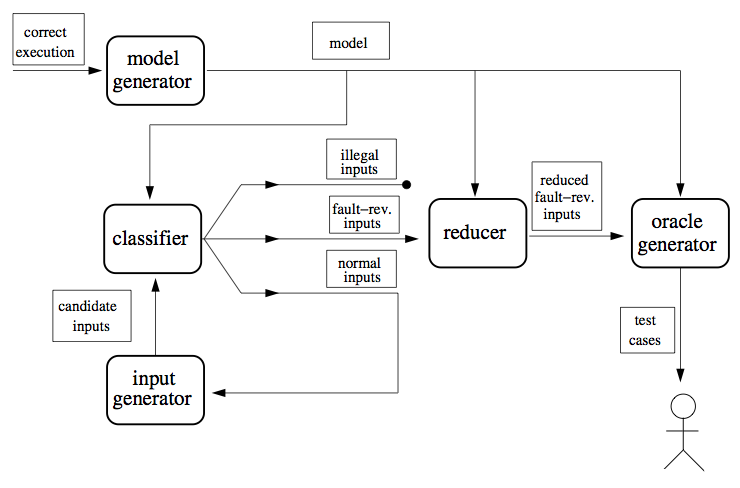
\includegraphics[width=15cm, height=10.5cm]{chapter2/eclat_working.png}
	\caption{The input selection technique. Implicit in the diagram is the program under test. Rectangles with rounded corners represent steps in the technique, and rectangles with square corners represent artifacts~\cite{pacheco2005eclat}}
	\label{fig:eclat}
\end{figure}


Csallner and Smaragdakis~\cite{pacheco2007randoop} compared Eclat with JCrasher by executing nine programs on  both tools. They reported that Eclat performed better than JCrasher. On the average, Eclat selected 5.0 inputs per run out of which 30\% revealed faults while JCrasher selected 1.13 inputs per run out of which 0.92\% revealed faults. The limitation of Eclat is dependence on initial pool of correct test cases. Existence of errors in the pool leads to the creation of wrong operational model which adversely affects the testing process.   

%\subsection{JTest}
%Parasoft Jtest is a commercial tool that automatically generates and execute unit tests. It can be easily integrated to Java IDEs like Eclipse where it provide two main functionalities, i.e. Static Analysis, Unit testing and code coverage. [25]
%In static analysis Jtest takes a complete project or set of classes as input and compares it with a list of built-in rules. The statement violating any of these rules is an error. It also suggests probable fixes for the detected fault.
%For unit testing it takes a class as an input and processes a number of scenarios against it to generate and execute unit tests. Once unit tests are executed they become the part of regression test for future reference.
%Jtest also shows the code coverage of the program by colour coding the statements that are not executed by the unit tests.


\subsection{Randoop}
Random tester for object oriented programs (Randoop) is the tool used for implementing FDRT technique~\cite{pacheco2007randoop}. Randoop is a fully automatic tool, capable of testing Java classes and .Net binaries. It takes a set of classes, contracts, filters and time limit as input and gives a suite of JUnit for Java and NUnit for .Net program as output. Each unit test in a test suite is a sequence of method calls (hereafter referred as sequence). Randoop builds the sequence incrementally by randomly selecting a public method from the class under test.  Arguments for these methods are selected from the predefined pool in case of primitive type and as sequence of null values in case of reference type. Randoop maintains two sets called \verb+ErrorSeqs+ and \verb+NonErrorSeqs+ to record the feedback. It extends \verb+ErrorSeqs+ set in case of contract or filter violation and \verb+NonErrorSeqs+ set when no violation is recorded in the feedback. The use of this dynamic feedback evaluation at runtime brings an object to an interesting state. On test completion, \verb+ErrorSeqs+ and \verb+NonErrorSeqs+ are produced as JUnit/NUnit test suite. In terms of coverage and number of faults discovered, Randoop using FDRT technique was compared with JCrasher and JavaPathFinder and 14 libraries of both Java and .Net were evaluated~\cite{visser2004test}. The results showed that Randoop achieved more branch coverage and better fault detection than JCrasher. 

\subsection{QuickCheck}
QuickCheck~\cite{claessen2011quickcheck} is a lightweight random testing tool used for testing of Haskell programs~\cite{hudak2007history}. Haskell is a functional programming language where programs are evaluated by using expressions rather than statements. Most of the functions in Haskell are pure except the IO functions, therefore QuickCheck mainly focuses on testing pure functions. QuickCheck is designed to have a simple domain-specific language of testable specifications embedded in Haskell. This language is used to define expected properties of the functions under test. %- for example, reversing a list with single element must result in the same list.\\ %(author check the definition of pure functions)\\

QuickCheck takes as inputs the function to be tested and properties of the program (Haskell functions). The tool uses built-in random generator to generate test data, but it is also capable to use custom built data generator. The tester-defined-properties must hold while executing the function on the generated test data. Any violation of the defined properties will indicate error in the function.



% The function is executed against the generated test data. The QuickCheck evaluates and declares a fault in the function where a test case violates the set properties.   



%\subsection{AgitarOne}
%AgitarOne is a commercial tool that automatically generates unit tests. It has a Junit Generator engine that can create 25,000 lines or more of Junit per hour [29]. It can be easily integrated into famous IDE like Eclipse. It takes as input, classes under test, time and optionally any knowledge or test cases that has a positive influence on the performance of the testing process. The generated Junit tests can be run from the same IDE and can also be used for later regression testing. The GUI interface is called a dashboard which provides in depth knowledge of the tests conducted, failures detected, alerts and the archieves of the tests conducted earlier. It also shows the coverage obtained after executing the Junits against the code under test.

\subsection{AutoTest} \label{autotest_2}
The AutoTest is used to test Eiffel language programs~\cite{ciupa2007automatic}. The Eiffel language uses the concept of contracts which is effectively utilized by AutoTest. For example, the auto generated inputs are filtered using pre-conditions and non complying test inputs are discarded. The post-conditions are used as test oracle to determine whether the test passes or fails. Beside automated testing the AutoTest also allows the tester to manually write the test cases to target specific section of the code. The AutoTest takes one or more methods/classes as inputs and automatically generate test input data according to the requirements of the methods or classes.
\bigskip
\begin{figure}[h]
	\centering
	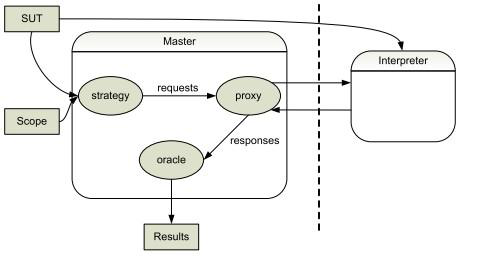
\includegraphics[width=14cm, height=8cm]{chapter2/autotest.png}
	\caption{AutoTest architecture~\cite{leitner2007reconciling}}
	\label{fig:autotest}
\end{figure}

\noindent As shown in Figure~\ref{fig:autotest}, the architecture of AutoTest can be split into the following four parts:
\begin{enumerate}
\item \textbf{Strategy:} It is a pluggable component where testers can fit any strategy according to the testing requirement. The strategy contains the directions for testing.%- for example what instructions should be executed on the SUT. Using the information the strategy synthesize test cases and forward it to the proxy. 
The default strategy creates random data to evaluate the methods/classes under test.
\item \textbf{Proxy:} It handles inter-process communication. The proxy receives execution requests from the strategy and forward these to the interpreter. It also sends the execution results to the oracle part.
\item \textbf{Interpreter:} It executes operations on the SUT. The most common operations include: create object, invoke routine and assign result. The interpreter is kept separate to increase robustness.
\item \textbf{Oracle:} It is based on contract-based testing. It evaluates the results to see if the contracts are satisfied. The outcome of the tests are formatted in HTML and stored on disk.
\end{enumerate}

\subsection{TestEra}
TestEra~\cite{marinov2001testera} is a novel framework for auto generation and evaluation of test inputs for a Java program. It takes specifications, numerical value and the method to be tested as input. It uses pre-conditions of a method to generate all non isomorphic valid test inputs to the specified limit. The test inputs are executed and the results are compared against the post-conditions of the method serving as oracle. Any test case that fails to satisfy post-condition is considered as a fault. 

\begin{figure}[h]
	\centering
	\centerline{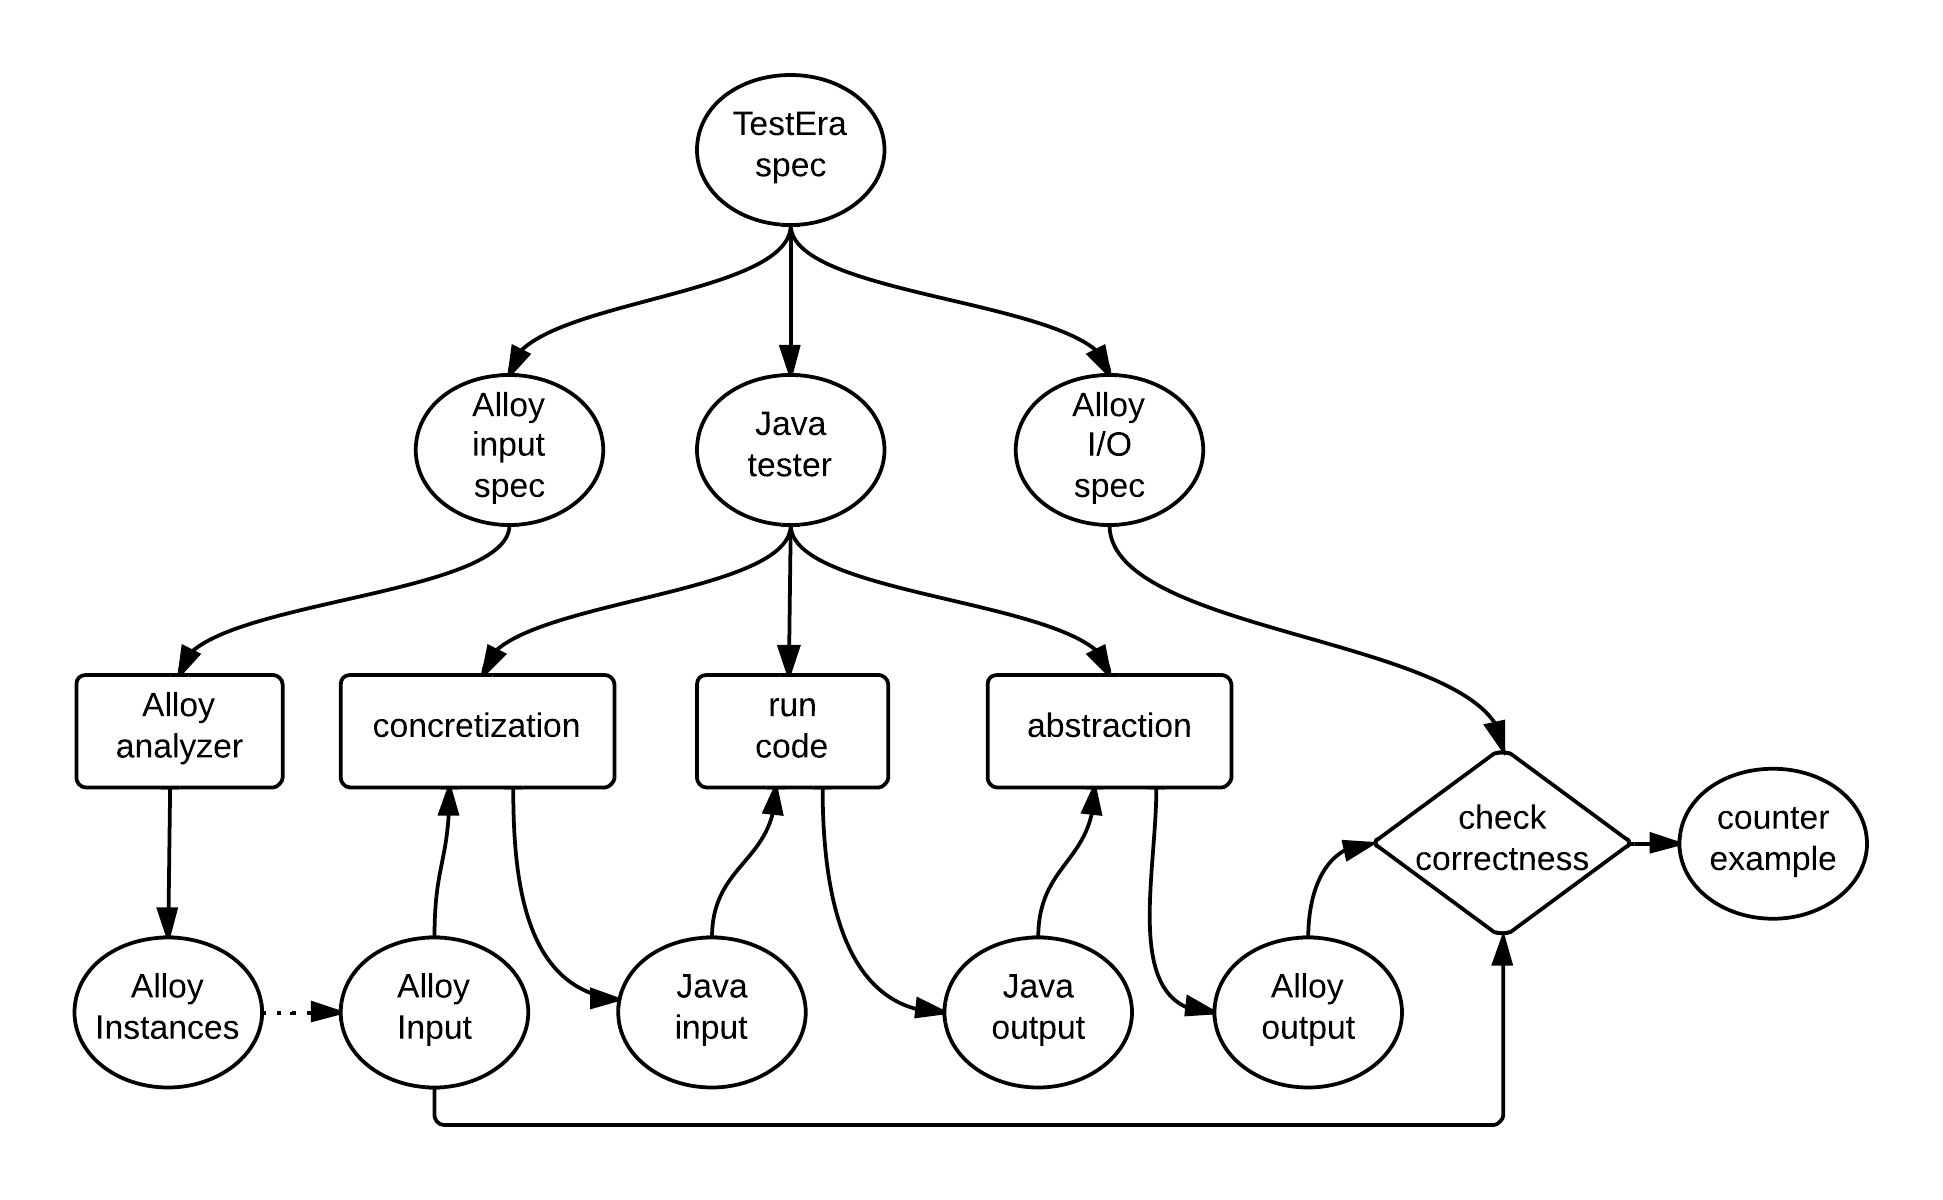
\includegraphics[width=15cm, height=10.7cm]{chapter2/TestEra.png}}
	\caption{TestEra framework~\cite{marinov2001testera}}
	\label{fig:testera}
\end{figure}

TestEra uses the Alloy modelling language~\cite{jackson2001micromodularity} to express constraints on test inputs and uses Alloy Analyser~\cite{jackson2000alcoa} to solve these constraints and generate test inputs. Alloy Analyzer performs the following three functions: (a) it translates Alloy predicates into propositional formulas%, i.e. constraints where all variables are boolean 
 (b) it evaluates the propositional formulas to find the outcome (c) it translates each outcome from propositional domain into the relational domain.




TestEra uses program specifications to guide the auto generation of test inputs as against Jartege (Section \ref{jartege_2}) and AutoTest (Section \ref{autotest_2}) which use program specifications for filtrating the irrelevant random generated test data. However, all the three tools use program specifications in a similar way for test oracle. 


%Testera use specifications to guide the automatic generation of test inputs. It uses Alloy language for specification and Alloy Analyser to generate all non-isomorphic instances for a given size according to the specification automatically. Then, TestEra translate the instances to Java input as test cases for the program under test. After executing the test, TestEra then translate the outputs back to Alloy and Alloy Analyzer check the input and output against the correctness criteria given in Alloy. When it detects a violation, TestEra generates report in the form of concrete counterexamples. Figure 2.6 [50] illustrates the basic framework of TestEra.

\subsection{Korat} % please read thesis of khurshid in Mendeley in phd thesis section for more information.
Korat~\cite{boyapati2002korat} like TestEra~\cite{marinov2001testera}, both developed by the same team, is a framework for automated testing of Java programs based on the formal specifications~\cite{chang1999structural}. Korat uses Java Modelling Language (JML) for specifications. It uses bounded-exhaustive testing in which the code is tested against all possible inputs within the specified bounds~\cite{khurshid2001checking}. %Korat generates structurally complex inputs by solving imperative predicates. An imperative predicate is a piece of code that takes a structure as input and evaluates it to a boolean value. 
Korat takes imperative predicates and finitization value as inputs. It systematically explores the input space of the predicates and generates all non-isomorphic inputs for which the predicates return true. The core part of Korat monitors execution of the predicates on candidate inputs to filter out the fields accessed during executions. These inputs are taken as test cases. 

Korat uses \verb+repOK()+ and \verb+checkRep()+ methods. The \verb+repOK()+ is used to check the class invariants for validating test inputs while \verb+checkRep()+ is used to verify the post-conditions for validating the test case. Korat does not require existing set of operations to create input values. Therefore it has the advantage of generating input values that may be difficult or impossible with a given set of operations. The disadvantage of the approach is the requirement of significant manual efforts \cite{pacheco2009directed}.    

%As the test start, it uses methods pre-condition to generate all non-isomorphic test cases up to a given size. It then executes each of the test case and compare the obtained results to the methods post-condition, which serves as an oracle to evaluate the correctness of each test case. 

\subsection{Yeti}
York Extensible Testing Infrastructure (YETI) is an open-source automated random testing tool. YETI, coded in Java, is capable of testing systems developed in procedural, functional and object-oriented languages. Its language agnostic meta-model enables it to test programs written in multiple languages including Java, C\#, JML and .NET. The core features of YETI include easy extensibility for future growth, capability to test programs using multiple strategies, high speed tests execution, real time logging, GUI support and auto generation of test report at the end of test session. Detailed information about YETI is presented in Chapter \ref{chap:yeti_3}.





%\section{Automated Random Testing}
%\subsection{Test Data Generation}
%\subsection{Test Execution}



%\subsection{Test Report}

\section{Summary}
The software testing is summarized graphically with the help of two dimensional venn diagram as shown in Figure~\ref{fig:testDataGenerators_2}. The positive x-axis represent black-box while negative x-axis represent white-box testing. Similarly on positive y axis we have dynamic testing and on negative y axis we have static testing. If a testing technique is black-box and dynamic then it will fall in 0 to 90 degree and if it is black-box and static it will fall in 270 to 360 degree. On the other hand if the test is white-box and dynamic then it will fall in 90 to 180 degree and if the test is white-box and static then it will fall in 180 to 270 degrees.

\begin{figure}[h]
	\centering
	\centerline{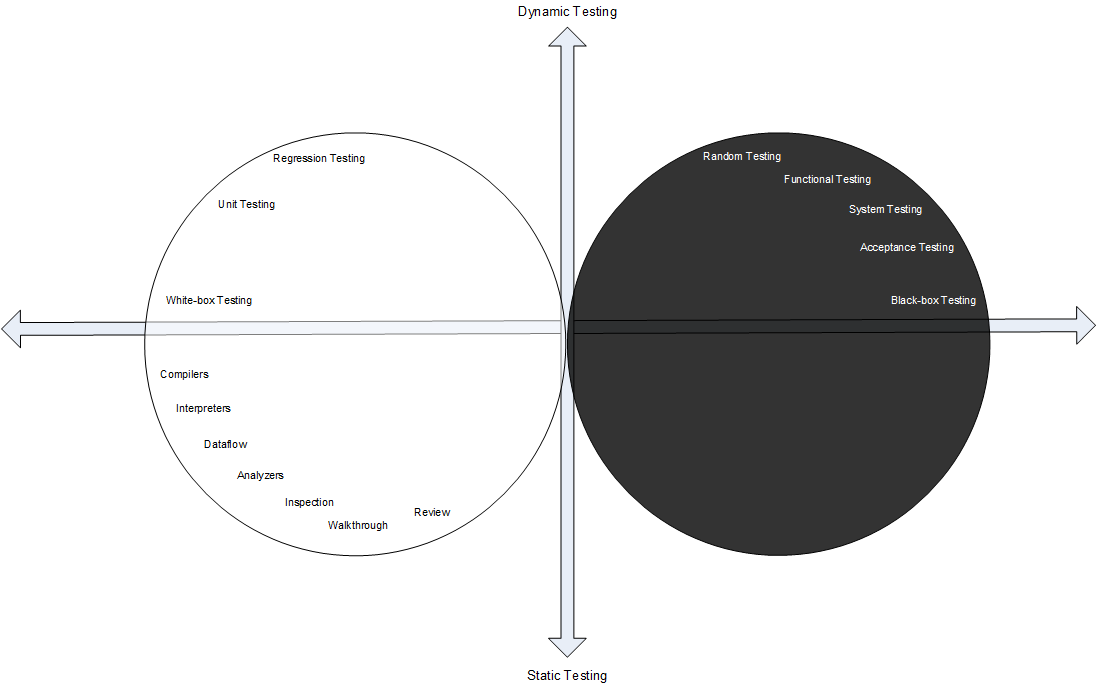
\includegraphics[width=16cm, height=12cm ]{chapter2/DrawingTesting.png}}
	\caption{Types of software testing}
	\label{fig:testDataGenerators_2}
\end{figure}


The chapter gives an overview of software testing, including definition, common types, need, purpose and uses. It differentiates manual and automated software testing and describes various ways of software test data generation, being the crucial part of any testing system. The later part describes random testing and the various ways of improving the performance of random testing. Finally, information is presented on how the automated testing tools implement random technique for software testing. Main features of automatic testing tools used in random testing are summarized in Figure~\ref{fig:Tools}.

%\begin{figure}[H]
%	\centering
%	%\centerline{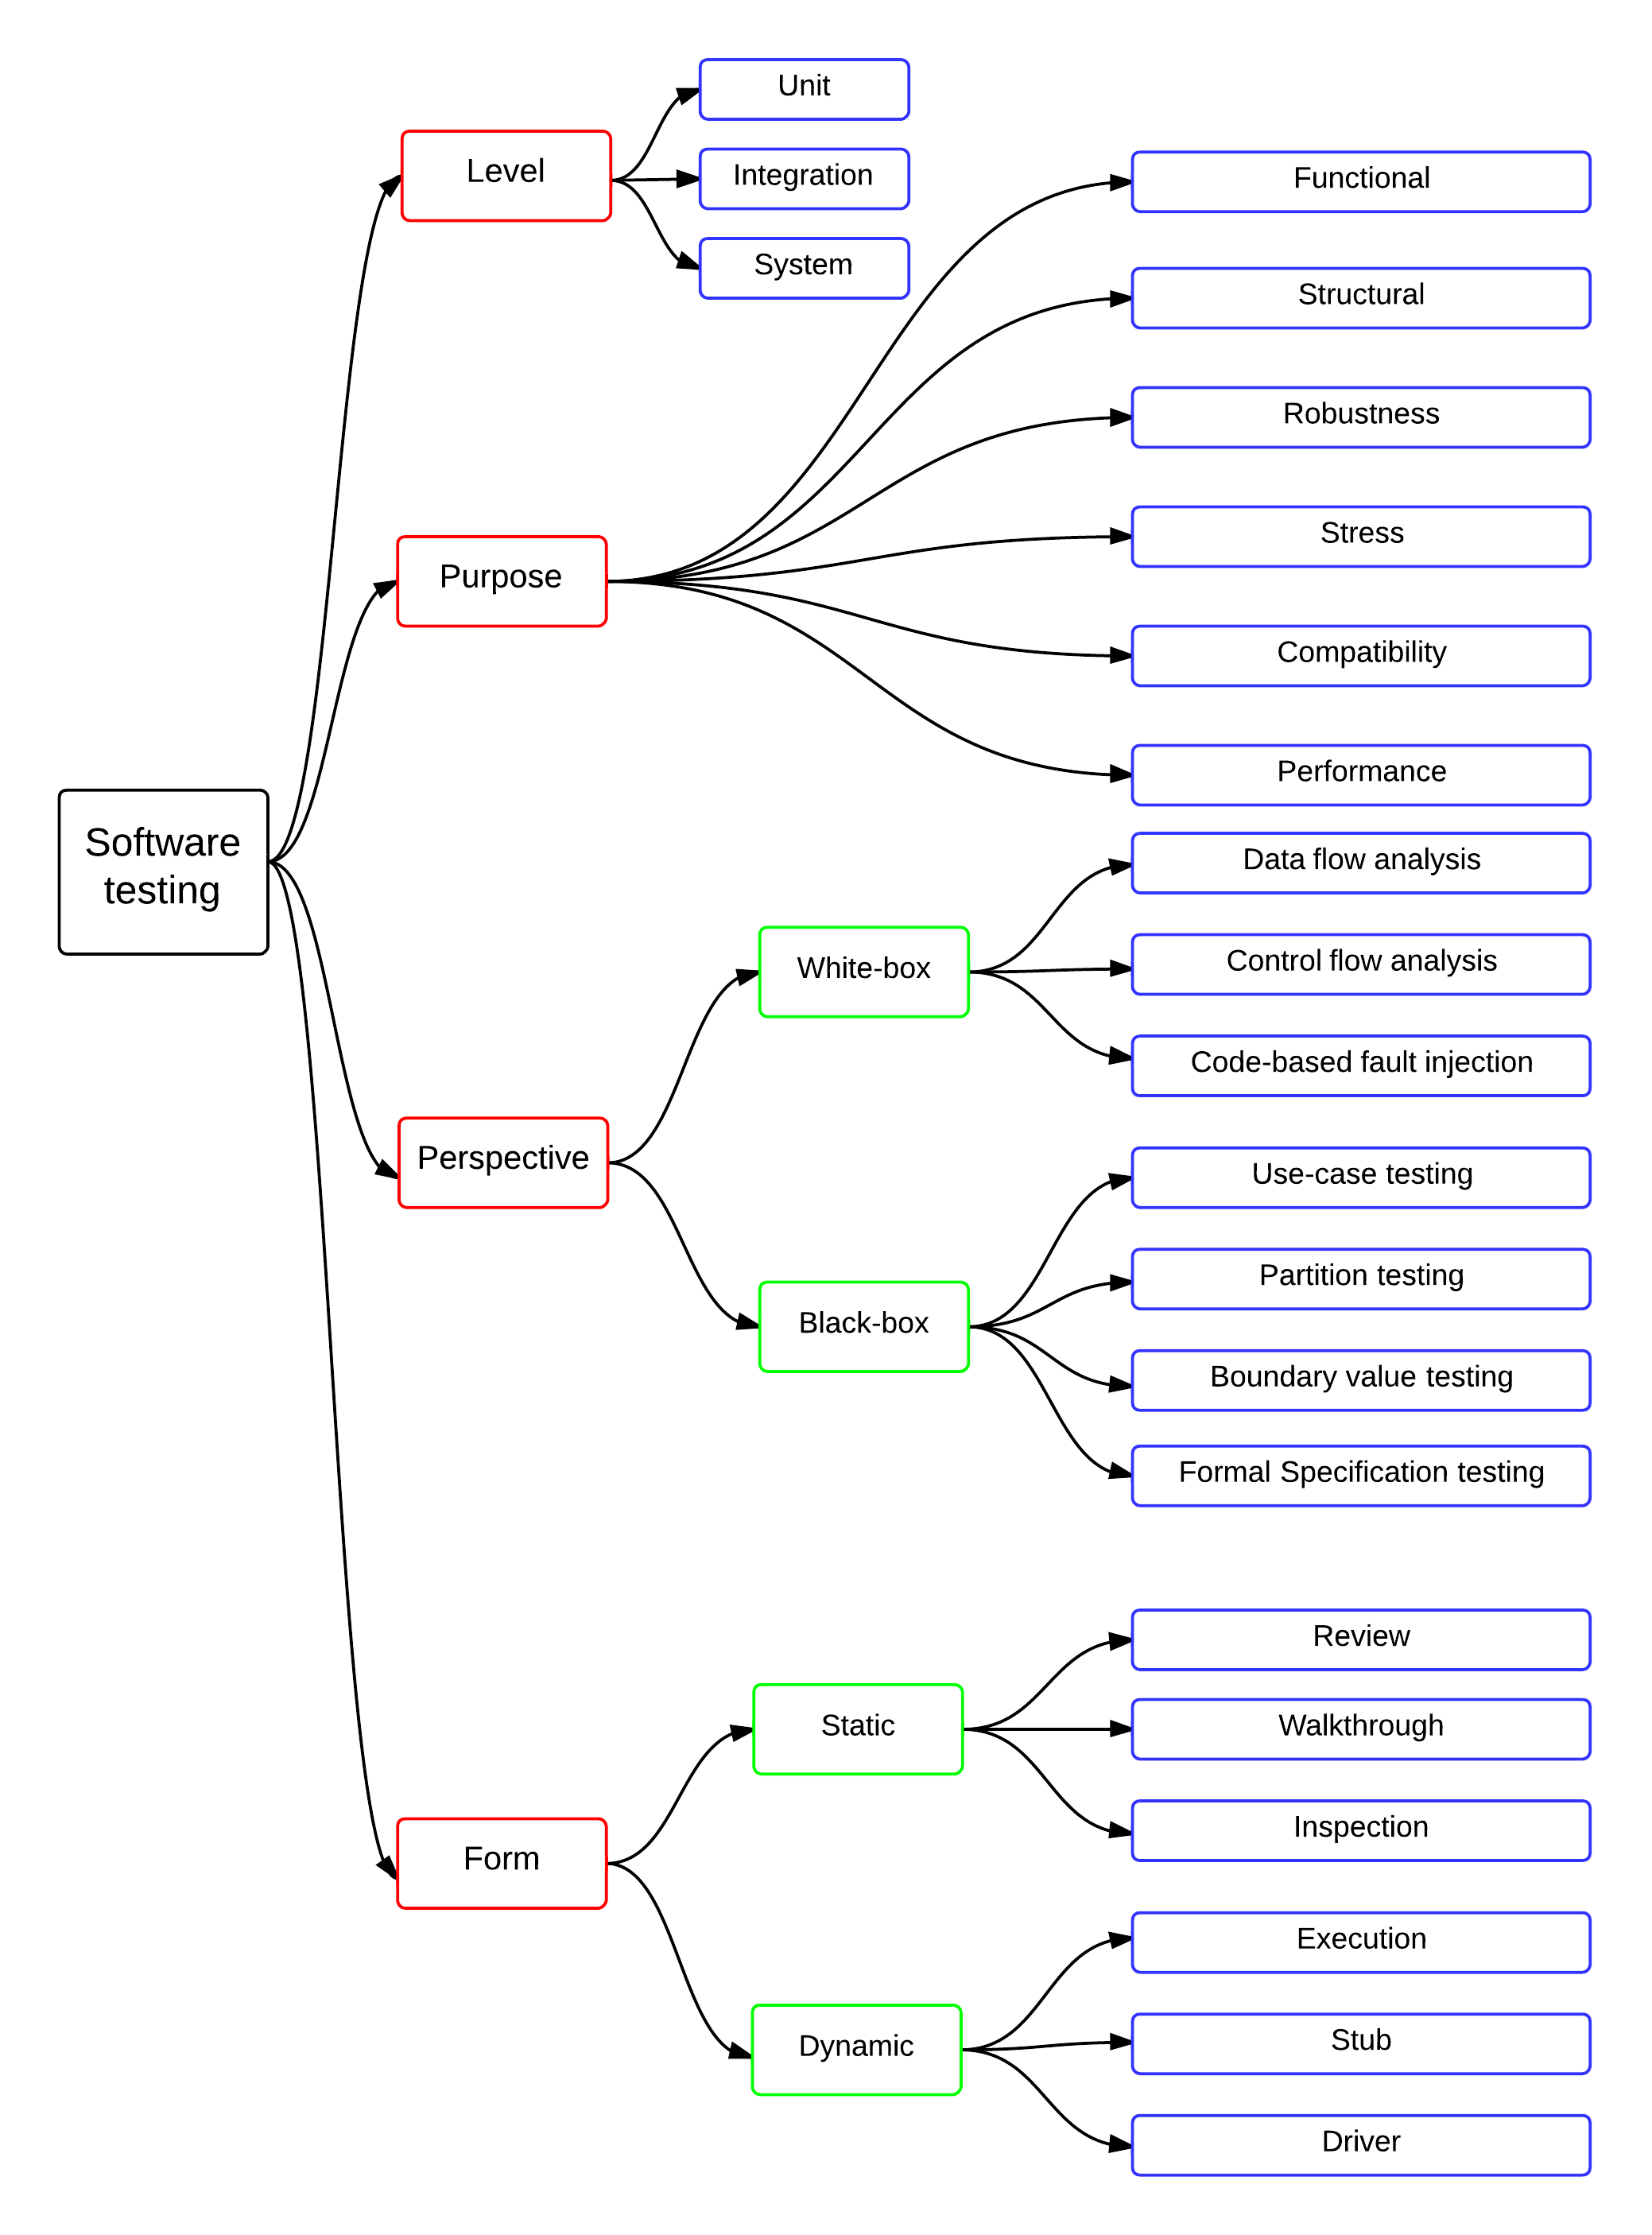
\includegraphics[width=16cm, height=16cm]{chapter2/softwareTestingFlow.png}}
%	%\centerline{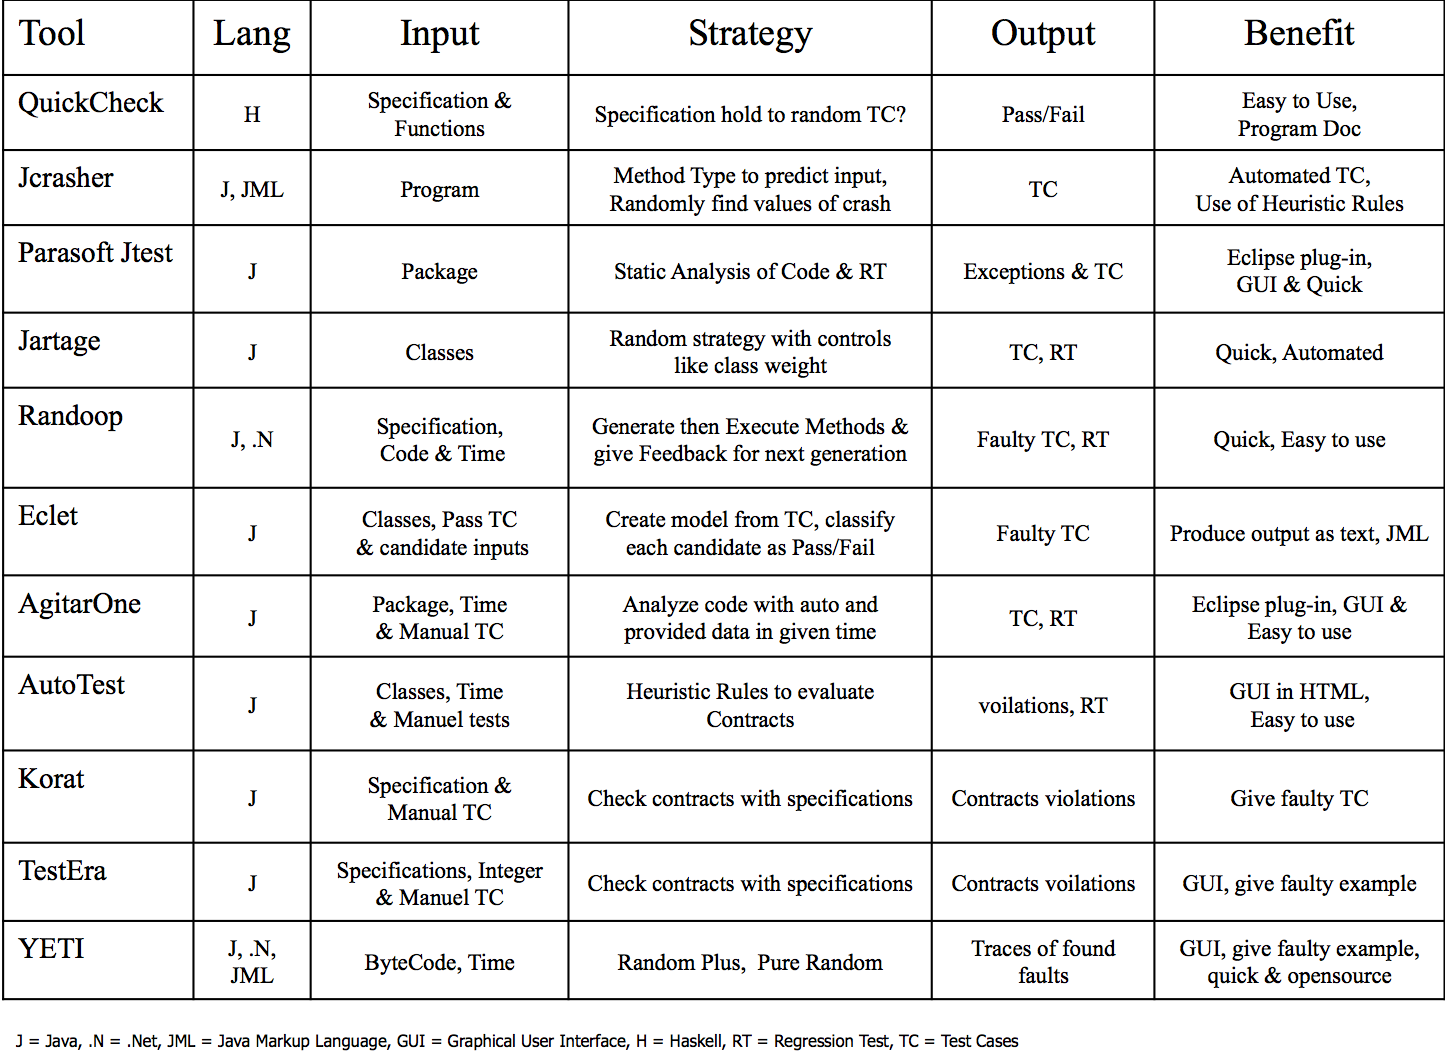
\includegraphics[width=15.5cm, height=15cm]{chapter2/Tools.png}}
%	\centerline{\includegraphics[width=17.5cm, height=15cm]{chapter2/RandomTools01.png}}
%	\caption{Main features of automatic testing tools using random testing}
%	\label{fig:Tools}
%\end{figure}


\begin{sidewaysfigure}[htp]
\centering
\centerline{\includegraphics[width=26cm, height=15cm]{chapter2/RandomTools01.png}}
	\caption{Main features of automatic testing tools using random testing}
	\label{fig:Tools}
\end{sidewaysfigure}

%\begin{figure}[H]
%	\centering
%	%\centerline{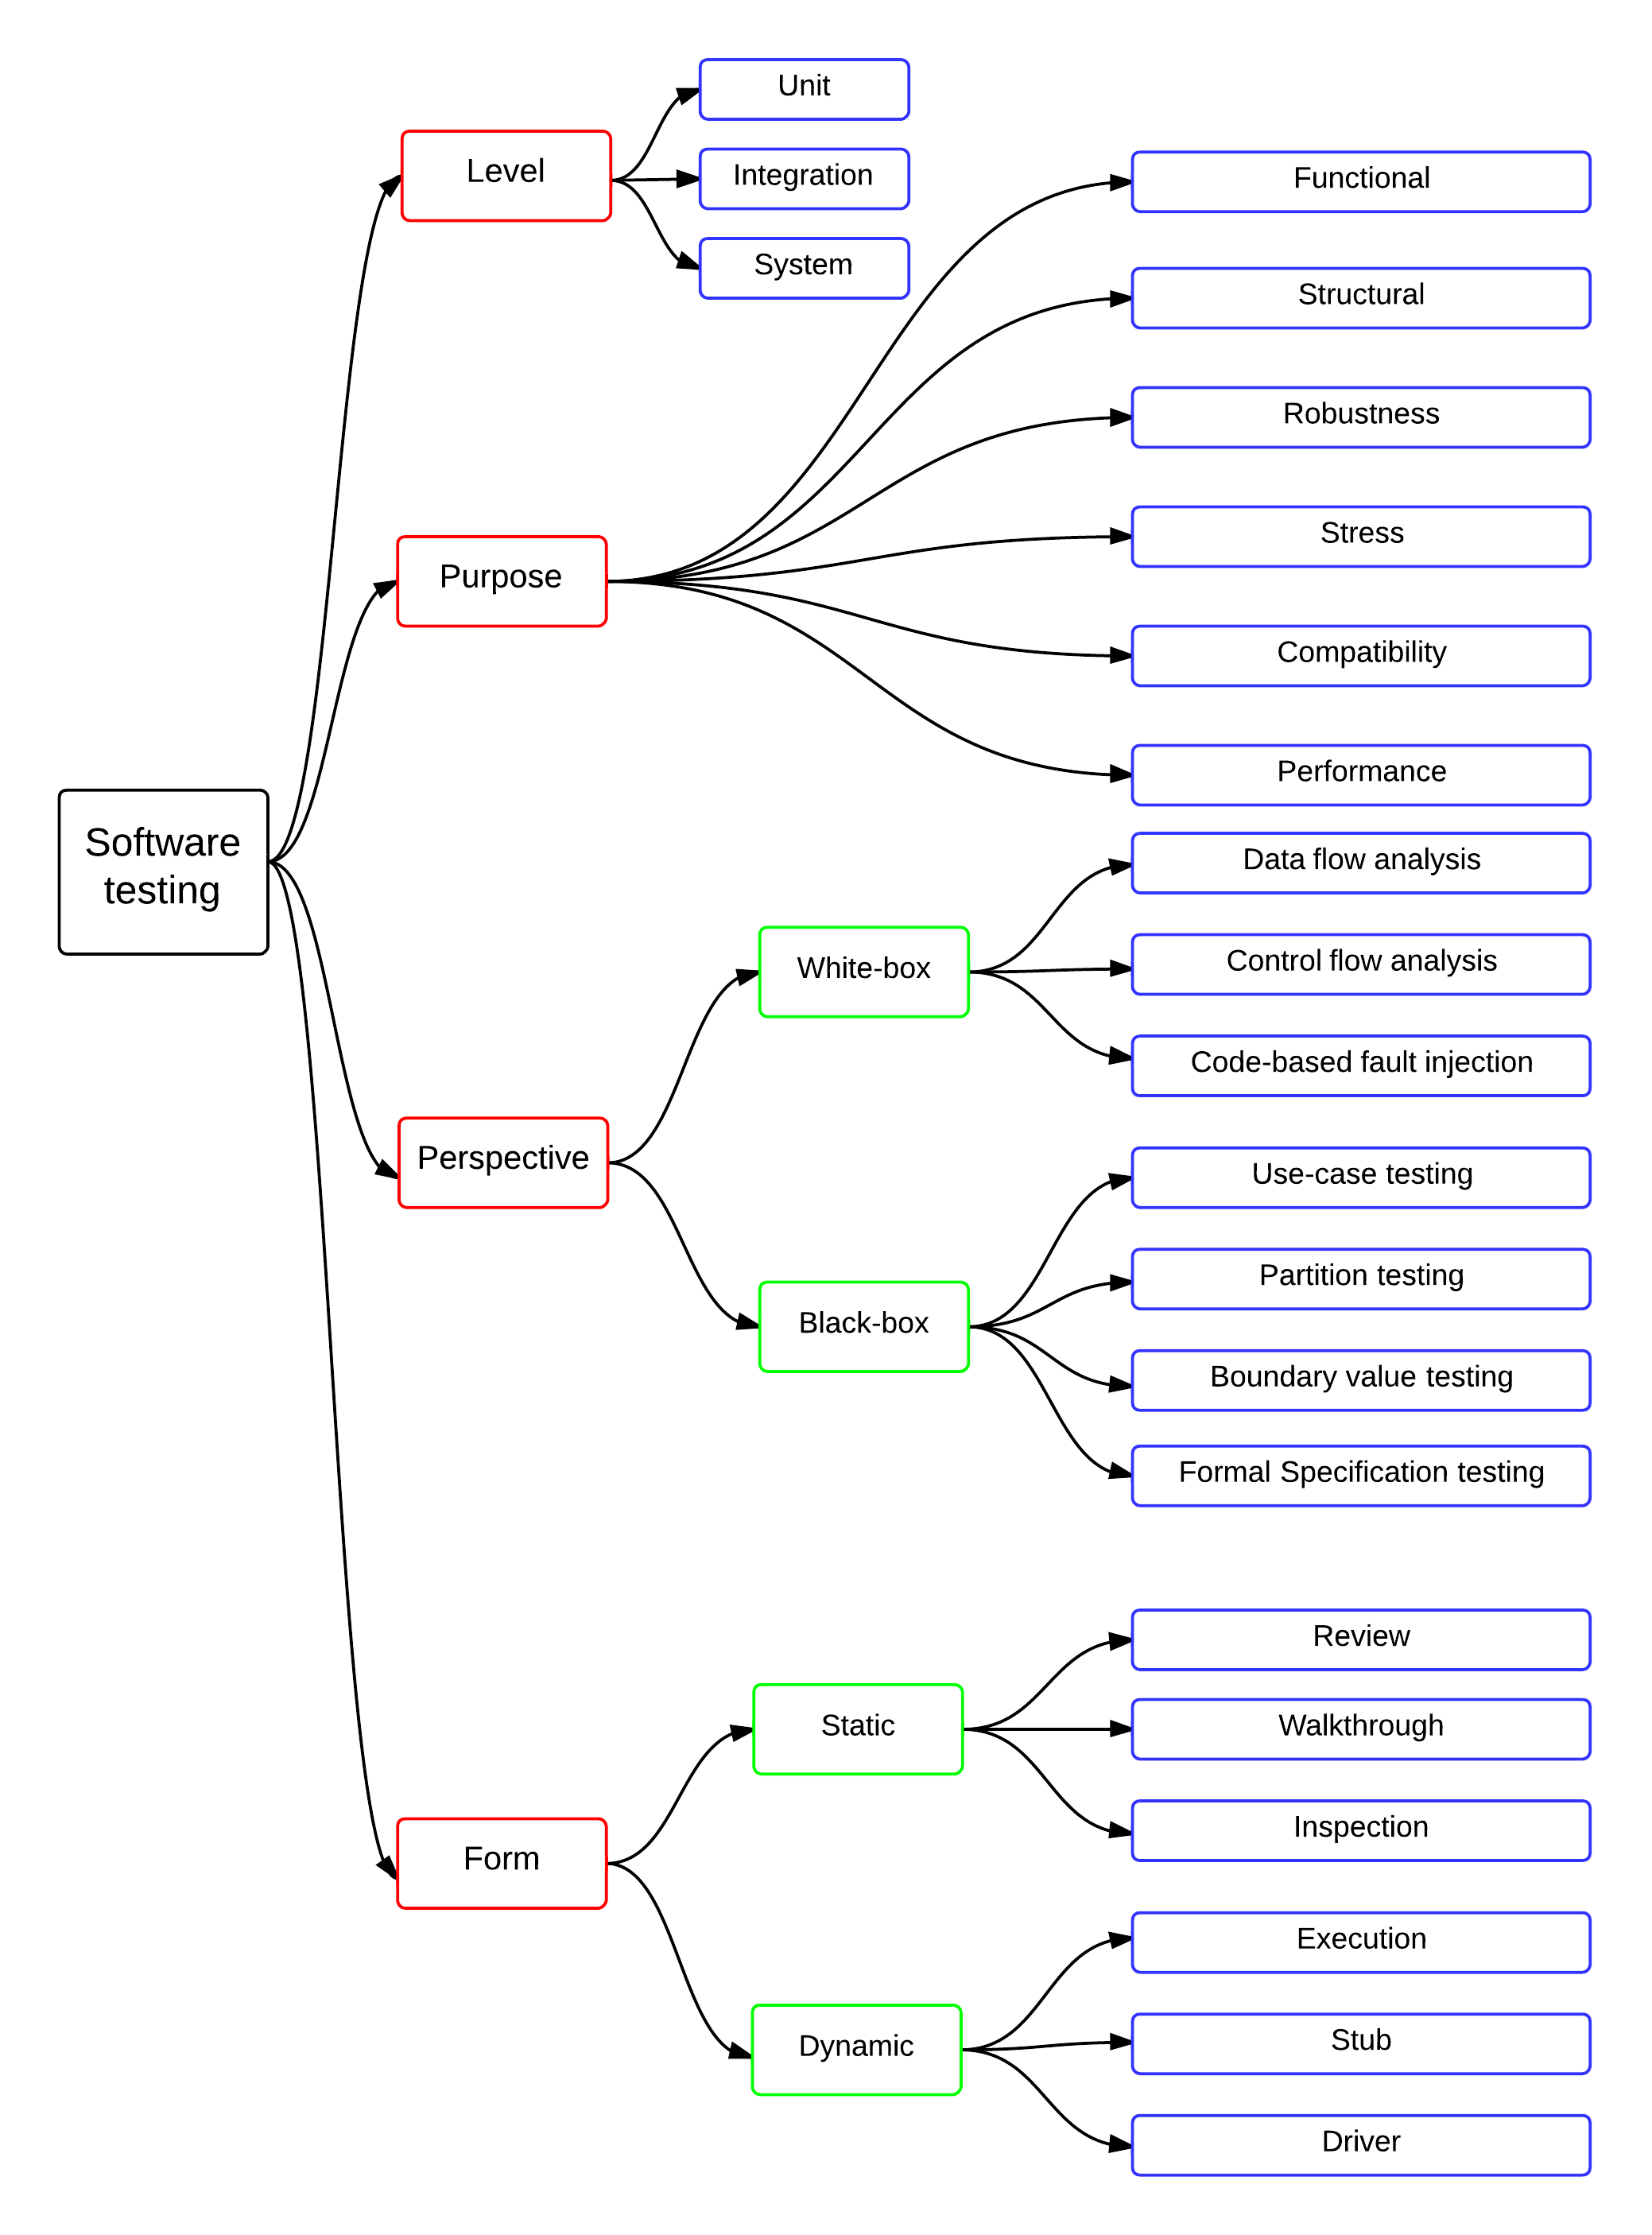
\includegraphics[width=16cm, height=16cm]{chapter2/softwareTestingFlow.png}}
%	\centerline{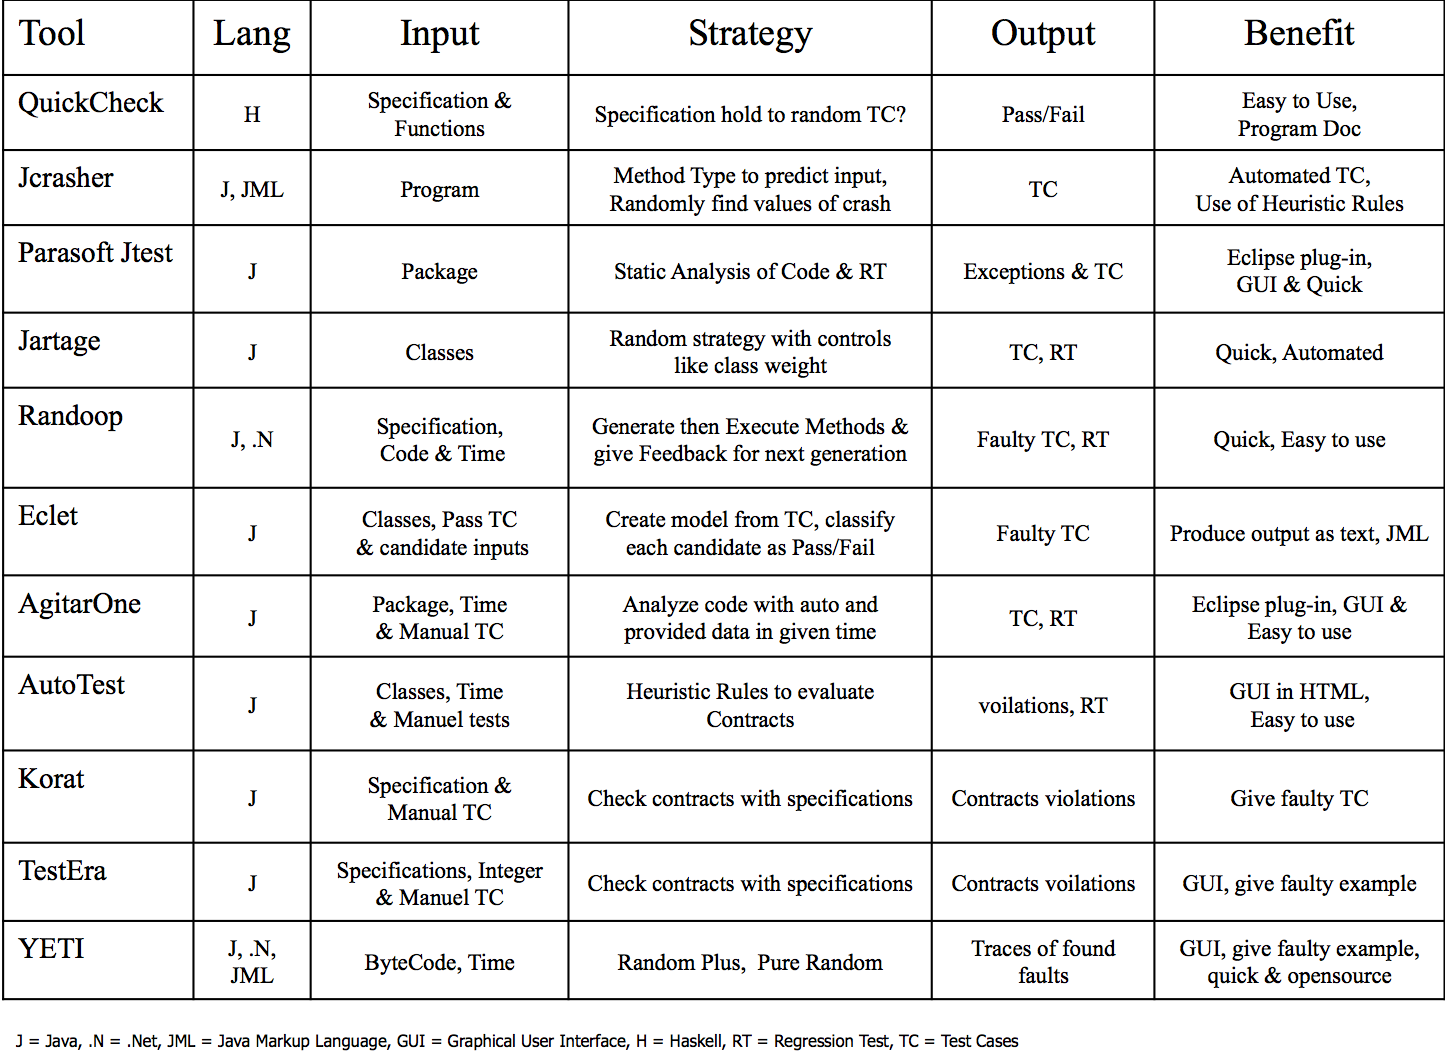
\includegraphics[width=15.5cm, height=15cm]{chapter2/Tools.png}}
%	\caption{Main features of automatic testing tools used in random testing}
%	\label{fig:Tools}
%\end{figure}





%\begin{sidewaystable}
%    \centering
%    \caption{Main features of automatic testing tools used in random testing}
%    \bigskip
%   \begin{tabular}{|l|l|l|l|l|l|}
%\hline

%Tool 				& Language																								& Input  																																			& Strategy 																																											 				& Output		  																								& Benefits																															\\ \hline
%JCrasher	  & Java, JML																								& Program																																			& \vtop{\hbox{\strut Method type to predict input,}\hbox{\strut Randomly find values of crash}}  				& TC																													& \vtop{\hbox{\strut Automated TC, Use} \hbox{of Heuristic Rules}} 	 \\ \hline
%Jartege			& Java																										& Classes																																			& \vtop{\hbox{\strut Random strategy with controls}\hbox{\strut like weight etc.}} 							 				& TC, RT 																											& Quick, automated																									 \\ \hline
%Eclat				& Java																										& Classes, pass TC 																														& \vtop{\hbox{\strut Create model from TC, execute}\hbox{\strut each candidate on the model}} 					& Faulty TC 																									& \vtop{\hbox{\strut produce output text,} \hbox{JML}}									\\ \hline
%Quickcheck	& Haskell																									&	\vtop{\hbox{\strut Specifications}  \hbox{\strut and Functions}}	  			  & \vtop{\hbox{\strut Specification} \hbox{\strut hold to random TC?}} 											 						& Pass/Fail																										& \vtop{\hbox{\strut Easy to use, program} \hbox{documentation}}				\\ \hline
%Randoop 		& Java, .NET																							& \vtop{\hbox{\strut Specifications,} \hbox{\strut code and time}}					  & \vtop{\hbox{\strut Generate and execute methods} \hbox{\strut \& give feedback for next generation}} 	& Fault TC, RT 																								& 																																\\ \hline
%AgitarOne		& Java																										& \vtop{\hbox{\strut Package, time}   \hbox{\strut and manual TC}}						& \vtop{\hbox{\strut Analyse SUT with auto and} \hbox{\strut provided data in specified time}} 					& TC, RT																											& \vtop{\hbox{\strut Eclipse plug-in} \hbox{\& easy to use}}  			 \\ \hline
%AutoTest		& Java																										& \vtop{\hbox{\strut Classes, time}   \hbox{\strut and manual TC}} 						& \vtop{\hbox{\strut Heuristic rules} \hbox{\strut to evaluate contracts}} 															& violations, RT 																							& \vtop{\hbox{\strut GUI in HTML,} \hbox{easy to use}} 								\\ \hline
%TestEra			& Java																										& \vtop{\hbox{\strut Specifications,} \hbox{\strut integer \& manual TC}}			& \vtop{\hbox{\strut Check contracts} \hbox{\strut with specifications}} 																& Contracts violations 																				& \vtop{\hbox{\strut short report with} \hbox{faulty TC only}} 					\\ \hline
%Korat 			& Java																										& \vtop{\hbox{\strut Specifications}  \hbox{\strut and manual tests}}					& \vtop{\hbox{\strut Check contracts} \hbox{\strut with specifications}}																& Contracts violations 																				& \vtop{\hbox{\strut GUI, short report} \hbox{with faulty TC only}} 	 \\ \hline
%YETI 				& \vtop{\hbox{\strut Java, .NET,}  \hbox{\strut JML}} 		& Code, Time 																																  & RandomPlus, Random 																																										& \vtop{\hbox{\strut Traces of found } \hbox{\strut faults}}	& \vtop{\hbox{\strut GUI, give faulty} \hbox{examples, Quick}} 			 \\ \hline %inserts single line
%\end{tabular}
%\label{table:Tools}
%\end{sidewaystable}

% ------------------------------------------------------------------------


%%% Local Variables:
%%% mode: latex
%%% TeX-master: "../thesis"

%%% End:
